%%%%%%%% ICML 2019 EXAMPLE LATEX SUBMISSION FILE %%%%%%%%%%%%%%%%%

\documentclass{article}

% Recommended, but optional, packages for figures and better typesetting:

\usepackage{caption}
\usepackage{amsthm}
\usepackage{tabularx}
\usepackage{bm}
\usepackage{array}
\usepackage{balance}
\usepackage{amsmath}
\usepackage{amssymb}
\usepackage{multirow}
\usepackage{color}
\usepackage{microtype}
\usepackage{graphicx}
\usepackage{subfigure}
\usepackage{booktabs}
\usepackage{bbm}

\def\rc{\color{red}}
\def\bc{\color{blue}}

\usepackage[colorlinks,linkcolor=red,citecolor=blue]{hyperref}       % hyperlinks
\usepackage{natbib}
\allowdisplaybreaks

\DeclareMathOperator*{\Argmax}{Argmax}
\DeclareMathOperator*{\Argmin}{Argmin}

\newcommand{\var}{{\rm var}}
\newcommand{\Tr}{^{\rm T}}
\newcommand{\vtrans}[2]{{#1}^{(#2)}}
\newcommand{\kron}{\otimes}
\newcommand{\schur}[2]{({#1} | {#2})}
\newcommand{\schurdet}[2]{\left| ({#1} | {#2}) \right|}
\newcommand{\had}{\circ}
\newcommand{\diag}{{\rm diag}}
\newcommand{\invdiag}{\diag^{-1}}
\newcommand{\rank}{{\rm rank}}
\newcommand{\expt}[1]{\langle #1 \rangle}
% careful: ``null'' is already a latex command
\newcommand{\nullsp}{{\rm null}}
\newcommand{\tr}{{\rm tr}}
\renewcommand{\vec}{{\rm vec}}
\newcommand{\vech}{{\rm vech}}
\renewcommand{\det}[1]{\left| #1 \right|}
\newcommand{\pdet}[1]{\left| #1 \right|_{+}}
\newcommand{\pinv}[1]{#1^{+}}
\newcommand{\erf}{{\rm erf}}
\newcommand{\hypergeom}[2]{{}_{#1}F_{#2}}
\newcommand{\mcal}[1]{\mathcal{#1}}
\newcommand{\Rcal}{{\mathcal{R}}}
\newcommand{\Acal}{{\mathcal{A}}}
\newcommand{\Ccal}{{\mathcal{C}}}
\newcommand{\Fcal}{{\mathcal{F}}}
% boldface characters
\renewcommand{\a}{{\bf a}}
\renewcommand{\b}{{\bf b}}
\renewcommand{\c}{{\bf c}}
\renewcommand{\d}{{\rm d}}  % for derivatives
\newcommand{\e}{{\bf e}}
\newcommand{\f}{{\bf f}}
\newcommand{\g}{{\bf g}}
\newcommand{\h}{{\bf h}}
\newcommand{\bi}{{\bf i}}
\newcommand{\bj}{{\bf j}}
\newcommand{\bK}{{\bf K}}
\newcommand{\Kcal}{{\mathcal{K}}}
% in Latex2e this must be renewcommand
\renewcommand{\k}{{\bf k}}
\newcommand{\m}{{\bf m}}
\newcommand{\mhat}{{\overline{m}}}
\newcommand{\tm}{{\tilde{m}}}
\newcommand{\n}{{\bf n}}
\renewcommand{\o}{{\bf o}}
\newcommand{\p}{{\bf p}}
\newcommand{\q}{{\bf q}}
\renewcommand{\r}{{\bf r}}
\newcommand{\s}{{\bf s}}
\renewcommand{\t}{{\bf t}}
\renewcommand{\u}{{\bf u}}
\renewcommand{\v}{{\bf v}}
\newcommand{\w}{{\bf w}}
\newcommand{\x}{{\bf x}}
\newcommand{\y}{{\bf y}}
\newcommand{\z}{{\bf z}}
\newcommand{\bl}{{\bf l}}
\newcommand{\A}{{\bf A}}
\newcommand{\B}{{\bf B}}
\newcommand{\C}{{\bf C}}
\newcommand{\D}{{\bf D}}
\newcommand{\Dcal}{\mathcal{D}}
\newcommand{\E}{{\bf E}}
\newcommand{\F}{{\bf F}}
\newcommand{\G}{{\bf G}}
\newcommand{\Gcal}{{\mathcal{G}}}
\renewcommand{\H}{{\bf H}}
\newcommand{\I}{{\bf I}}
\newcommand{\J}{{\bf J}}
\newcommand{\K}{{\bf K}}
\renewcommand{\L}{{\bf L}}
%\newcommand{\Lcal}{{\mathcal{L}}}
\newcommand{\M}{{\bf M}}
\newcommand{\Mcal}{{\mathcal{M}}}
\newcommand{\N}{\mathcal{N}}  % for normal density
%\newcommand{\N}{{\bf N}}
\newcommand{\bupeta}{\boldsymbol{\upeta}}
\renewcommand{\O}{{\bf O}}
\renewcommand{\P}{{\bf P}}
\newcommand{\Q}{{\bf Q}}
\newcommand{\R}{{\bf R}}
\renewcommand{\S}{{\bf S}}
\newcommand{\Scal}{{\mathcal{S}}}
\newcommand{\T}{{\bf T}}
\newcommand{\Tcal}{{\mathcal{T}}}
\newcommand{\U}{{\bf U}}
\newcommand{\Ucal}{{\mathcal{U}}}
\newcommand{\tU}{{\tilde{\U}}}
\newcommand{\tUcal}{{\tilde{\Ucal}}}
\newcommand{\V}{{\bf V}}
\newcommand{\W}{{\bf W}}

\newcommand{\Ocal}[1]{{\mathcal{O}\left( #1  \right)}}
\newcommand{\Omegacal}[1]{{\Omega \left( #1 \right)}}
\newcommand{\Pcal}{{\mathcal{P}}}
\newcommand{\Hcal}{{\mathcal{H}}}
\newcommand{\Wcal}{{\mathcal{W}}}
\newcommand{\X}{{\bf X}}
\newcommand{\Xcal}{{\mathcal{X}}}
\newcommand{\Y}{{\bf Y}}
\newcommand{\Ycal}{{\mathcal{Y}}}
\newcommand{\Z}{{\bf Z}}
\newcommand{\Zcal}{{\mathcal{Z}}}

% this is for latex 2.09
% unfortunately, the result is slanted - use Latex2e instead
%\newcommand{\bfLambda}{\mbox{\boldmath$\Lambda$}}
% this is for Latex2e
\newcommand{\bfLambda}{\boldsymbol{\Lambda}}

% Yuan Qi's boldsymbol
\newcommand{\bsigma}{\boldsymbol{\sigma}}
\newcommand{\balpha}{\boldsymbol{\alpha}}
\newcommand{\bpsi}{\boldsymbol{\psi}}
\newcommand{\bphi}{\boldsymbol{\phi}}
\newcommand{\bbeta}{\boldsymbol{\beta}}
\newcommand{\bepsi}{\boldsymbol{\epsilon}}
\newcommand{\Beta}{\boldsymbol{\eta}}
\newcommand{\btau}{\boldsymbol{\tau}}
\newcommand{\bvarphi}{\boldsymbol{\varphi}}
\newcommand{\bzeta}{\boldsymbol{\zeta}}

\newcommand{\blambda}{\boldsymbol{\lambda}}
\newcommand{\bLambda}{\mathbf{\Lambda}}

\newcommand{\btheta}{\boldsymbol{\theta}}
\newcommand{\bTheta}{\boldsymbol{\Theta}}
\newcommand{\bpi}{\boldsymbol{\pi}}
\newcommand{\bxi}{\boldsymbol{\xi}}
\newcommand{\bSigma}{\boldsymbol{\Sigma}}
\newcommand{\bPi}{\boldsymbol{\Pi}}
\newcommand{\bOmega}{\boldsymbol{\Omega}}
%\newcommand{\bLambda}{\boldsymbol{\Lambda}}

\newcommand{\hatu}{\hat{\bf u}}



\newcommand{\bgamma}{\boldsymbol{\gamma}}
\newcommand{\bGamma}{\boldsymbol{\Gamma}}
\newcommand{\bUpsilon}{\boldsymbol{\Upsilon}}



\newcommand{\bmu}{\boldsymbol{\mu}}
\newcommand{\1}{{\bf 1}}
\newcommand{\0}{{\bf 0}}


\newcommand{\proj}[1]{{\rm proj}\negmedspace\left[#1\right]}
\newcommand{\argmin}{\operatornamewithlimits{argmin}}
\newcommand{\argmax}{\operatornamewithlimits{argmax}}

\newcommand{\dif}{\mathrm{d}}
\newcommand{\lrincir}[1]{\left( #1 \right)}
\newcommand{\abs}[1]{\lvert#1\rvert}
\newcommand{\norm}[1]{\lVert#1\rVert}
\newcommand{\lrnorm}[1]{\left\lVert#1\right\rVert}
\newcommand{\lrangle}[1]{\left\langle#1 \right\rangle}

\newcommand{\ie}{{{i.e.,}}\xspace}
\newcommand{\eg}{{{\em e.g.,}}\xspace}
\newcommand{\EE}{\mathop{\mathbb{E}}}
\newcommand{\RR}{\mathbb{R}}
\newcommand{\sbr}[1]{\left[#1\right]}
\newcommand{\rbr}[1]{\left(#1\right)}
\newcommand{\Lcal}[1]{\mathcal{L}^{#1}_{D_1,D_2}}


\newcommand{\refabove}[2]{\displaystyle_{#1}^{(#2)}}
\newcommand{\refabovecir}[2]{\displaystyle_{#1}^{#2}}



 \newtheorem{Definition}{\bf{Definition}}
 \newtheorem{Theorem}{\bf{Theorem}}
 \newtheorem{reTheorem}[Theorem]{\bf{Theorem}}
 \newtheorem{Lemma}{\bf{Lemma}}
 \newtheorem{reLemma}[Lemma]{\bf{Lemma}}
 \newtheorem{Corollary}{\bf{Corollary}}
 \newtheorem{reCorollary}[Corollary]{\bf{Corollary}}
 \newtheorem{Assumption}{\bf{Assumption}}
 \newtheorem{Proposition}{\bf{Proposition}}
 \newtheorem{Remark}{\bf{Remark}}



 % for professional tables

% hyperref makes hyperlinks in the resulting PDF.
% If your build breaks (sometimes temporarily if a hyperlink spans a page)
% please comment out the following usepackage line and replace
% \usepackage{icml2019} with \usepackage[nohyperref]{icml2019} above.
\usepackage{hyperref}

% Attempt to make hyperref and algorithmic work together better:
\newcommand{\theHalgorithm}{\arabic{algorithm}}

% Use the following line for the initial blind version submitted for review:
\usepackage{icml2019}

% If accepted, instead use the following line for the camera-ready submission:
%\usepackage[accepted]{icml2019}

% The \icmltitle you define below is probably too long as a header.
% Therefore, a short form for the running title is supplied here:
\icmltitlerunning{Decentralized Online Learning: Exchanging Local Models to Track Dynamics}

\begin{document}

\twocolumn[
\icmltitle{Decentralized Online Learning: Exchanging Local Models to Track Dynamics}

% It is OKAY to include author information, even for blind
% submissions: the style file will automatically remove it for you
% unless you've provided the [accepted] option to the icml2019
% package.

% List of affiliations: The first argument should be a (short)
% identifier you will use later to specify author affiliations
% Academic affiliations should list Department, University, City, Region, Country
% Industry affiliations should list Company, City, Region, Country

% You can specify symbols, otherwise they are numbered in order.
% Ideally, you should not use this facility. Affiliations will be numbered
% in order of appearance and this is the preferred way.
\icmlsetsymbol{equal}{*}

\begin{icmlauthorlist}
\icmlauthor{Aeiau Zzzz}{equal,to}
\icmlauthor{Bauiu C.~Yyyy}{equal,to,goo}
\icmlauthor{Cieua Vvvvv}{goo}
\icmlauthor{Iaesut Saoeu}{ed}
\icmlauthor{Fiuea Rrrr}{to}
\icmlauthor{Tateu H.~Yasehe}{ed,to,goo}
\icmlauthor{Aaoeu Iasoh}{goo}
\icmlauthor{Buiui Eueu}{ed}
\icmlauthor{Aeuia Zzzz}{ed}
\icmlauthor{Bieea C.~Yyyy}{to,goo}
\icmlauthor{Teoau Xxxx}{ed}
\icmlauthor{Eee Pppp}{ed}
\end{icmlauthorlist}

\icmlaffiliation{to}{Department of Computation, University of Torontoland, Torontoland, Canada}
\icmlaffiliation{goo}{Googol ShallowMind, New London, Michigan, USA}
\icmlaffiliation{ed}{School of Computation, University of Edenborrow, Edenborrow, United Kingdom}

\icmlcorrespondingauthor{Cieua Vvvvv}{c.vvvvv@googol.com}
\icmlcorrespondingauthor{Eee Pppp}{ep@eden.co.uk}

% You may provide any keywords that you
% find helpful for describing your paper; these are used to populate
% the "keywords" metadata in the PDF but will not be shown in the document
\icmlkeywords{Machine Learning, ICML}

\vskip 0.3in
]

% this must go after the closing bracket ] following \twocolumn[ ...

% This command actually creates the footnote in the first column
% listing the affiliations and the copyright notice.
% The command takes one argument, which is text to display at the start of the footnote.
% The \icmlEqualContribution command is standard text for equal contribution.
% Remove it (just {}) if you do not need this facility.

%\printAffiliationsAndNotice{}  % leave blank if no need to mention equal contribution
\printAffiliationsAndNotice{\icmlEqualContribution} % otherwise use the standard text.


\begin{abstract}
In this paper, we consider online learning in the decentralized setting up, which is motivated by the scenario where users want to take benefits from the data from other users, but do not want to share their private data to a third party or other users. Instead, they can only share their private prediction model, e.g., recommendation model. We study the decentralized online gradient method in which each user maintains a private model and share its private model with its neighbors (or users he/she trusts) periodically. In addition, to consider more practical scenario we allow users' interest changing over time, unlike most online work which assumes that the optimal prediction model is constant. We prove that decentralized online gradient can efficiently and effectively propagate the values in all private data without leaking them to track the dynamics, by admitting a tight dynamic regret $\Ocal{n\sqrt{TM}}$. Empirical studies are also conducted to validate our analysis.




\end{abstract}


\section{Introduction}
\label{sect_introduction}

For any online algorithm $A \in \Acal$, the previous dynamic regret $\widetilde{\Rcal}_T^{A}$ is defined by
\begin{align}
\label{equa_definition_previous_regret}
\widetilde{\Rcal}_T^{A} = &  \sum_{i=1}^n\sum_{t=1}^T \lrincir{ g_{i,t}(\x_{i,t}) - g_{i,t}(\x_t^\ast) },
\end{align} 





\paragraph{Notations and definitions}
In the paper, we make the following notations.
\begin{itemize}
\item For any $i\in[n]$ and $t\in[T]$, the random variable $\xi_{i,t}$ is subject to a distribution $D_t$, that is, $\xi_{i,t} \sim D_t$. Besides, a set of random variables $\Xi_{n,T}$ and the corresponding set of distributions are defined by
\begin{align}
\nonumber
\Xi_{n,T} = \{ \xi_{i,t} \}_{1\le i \le n, 1 \le t \le T}, \text{~and~} \Dcal_{T} = \{ D_t \}_{1 \le t \le T},
\end{align} respectively. For math brevity, we use the notation $\Xi_{n,T} \sim \Dcal_{T}$ to represent that $\xi_{i,t} \sim D_t$ holds for any $i\in[n]$ and $t\in[T]$. $\EE$ represents mathematical expectation.
\item For a decentralized network, we use $\W \in\RR^{n\times n}$ to represent its confusion matrix. It is a symmetric doublely stochastic matrix, which implies that every element of $\W$ is non-negative, $\W \1 = \1$, and $\1\Tr\W  = \1\Tr$. We use $\{\lambda_i\}_{i=1}^n$ with $\lambda_1 \ge \lambda_2 \ge \cdots \ge \lambda_n$ to represent its eigenvalues. 
\item $\partial$ and $\nabla$ represent sub-gradient and gradient operators, respectively. $\lrnorm{\cdot}$ represents the $\ell_2$ norm in default.
\item $\lesssim$ represents ``less than equal up to a constant factor".
\end{itemize} 
    











\section{Related work}
\label{sect_related_work}
Online learning has been studied for decades of years. The static regret of a sequential online convex optimization method can achieve $\Ocal{\sqrt{T}}$ and $\Ocal{\log T}$ bounds for convex and strongly convex loss functions, respectively \citep{Hazan2016Introduction,ShalevShwartz:2012dz}. Recently, both the decentralized online learing and the dynamic regret have drawn much attention due to their wide existence in the practical big data scenarios.
\subsection{Decentralized online learning}
Online learning in a decentralized network has been studied in \citep{8015179Shahram,Kamp:2014:CDO,Koppel-8352032,Zhang2018,pmlr-v70-zhang17g,Xu2015,tcns-7353155,cdc-7798923,acc-7172037,tcns-7479495,Benczur:2018ww,tkde-6311406}.  \citet{8015179Shahram} studies decentralized online mirror descent, and provides $\Ocal{n\sqrt{nTM}}$ dynamic regret. Here, $n$, $T$, and $M$ represent the number of nodes in the newtork, the number of iterations, and the budget of dynamics (defined in \eqref{equa_define_M}), respectively.  When the Bregman divergence in the decentralized online mirror descent is chosen appropriately, the decentralized online mirror descent becomes identical to the decentralized online gradient descent. Using the same definition of dynamic regret (defined in \eqref{equa_definition_previous_regret}), our method obtains $\Ocal{n\sqrt{TM}}$ dynamic regret for a decentralized online gradient descent, which is better than $\Ocal{n\sqrt{nTM}}$ in \citet{8015179Shahram}. The improvement of our bound benefits from a better bound of network error (see Lemma \ref{lemma_x_variance_norm_square}). \citet{Kamp:2014:CDO} studies decentralized online prediction, and presents $\Ocal{\sqrt{nT}}$ static regret.  It assumes that all data, used to yielded the loss, is generated from an unknown distribution. The strong assumption is not practical in the dynamic environment, and thus limits its novelity for a general online learning task. 
Additionally, many decentralized online optimization methods are proposed, for example, decentralized online multi-task learning \citep{Zhang2018}, decentralized online ADMM \citep{Xu2015}, decentralized online sub-gradient descent \citep{tcns-7353155}, decentralized continuous-time online saddle-point method \citep{cdc-7798923}, decentralized online  Nesterov's primal-dual method \citep{acc-7172037,tcns-7479495}. Those previous methods are proved to yield $\Ocal{\sqrt{T}}$ static regret, which do not have theoretical guarantee of regret in the dynamic environment.   Besides,  \citet{tkde-6311406} provides necessary and sufficient conditions to preserve privacy for decentralized online learning methods, which  is interesting to extend our method to be privacy-preserving in the future work.


\subsection{Regret in dynamic environment}

Dynamic regret has been widely studied for decades of years \citep{Zinkevich:2003,Hall:2015ct,Hall:2013vr,Jadbabaie:2015wg,Yang:2016ud,Bedi:2018te,Zhang:2016wl,Mokhtari:2016jz,Zhang:2018tu,Gyorgy:2016,NIPS2016_6536,Zhao:2018wx}.   \citet{Zinkevich:2003} first defines the dynamic regret by \eqref{equa_definition_previous_regret}, and then proposes an online gradient descent method. The method yields $\Ocal{\sqrt{TM}}$ by choosing an appropriate learning rate. The following researches achieve the sublinear dynamic regret, but extend the analysis of regret by using different reference points. For example, \citet{Hall:2015ct,Hall:2013vr} choose the reference points $\{\x_t^{\ast}\}_{t=1}^T$ satisfying $\sum_{t=1}^{T-1} \lrnorm{\x_{t+1}^\ast - \Phi(\x_t^\ast)} \le M$, where $\Phi(\x_t^\ast)$ is the predictive optimal decision variable. When the function $\Phi$ predicts accurately, a small $M$ is enough to bound the dynamics. The dynamic regret is thus effectively decreased. \citet{Jadbabaie:2015wg,Yang:2016ud,Bedi:2018te,Zhang:2016wl,Mokhtari:2016jz,Zhang:2018tu} chooses the reference points $\{\y_t^{\ast}\}_{t=1}^T$ with $\y_t^{\ast} = \argmin_{\z\in\Xcal} f_t(\z)$, where $f_t$ is the loss function at the $t$-th iteration. \citet{Gyorgy:2016} provides a new analysis framework, which achieves $\Ocal{\sqrt{TM}}$ dynamic regret\footnote{\citet{Gyorgy:2016} uses the notation of ``shifting regret" instead of ``dynamic regret". In the paper, we keep using ``dynamic regret" as used in most previous literatures. } for any given reference points. Besides, \citet{Zhao:2018wx} presents that the lower bound of the dynamic regret defined by \ref{equa_definition_previous_regret} is $\Omega\lrincir{\sqrt{TM}}$. The previous definition of the regret, i.e., \eqref{equa_definition_previous_regret}, is a special case of our new definition. When setting $\beta = 1$, we achieve the state-of-the-art regret, that is, $\Ocal{\sqrt{TM}}$. 

In some literatures, the regret in a dynamic environment is measured by the number of changes of a reference point over time. It is usually denoted by shifting regret or tracking regret \citep{Herbster1998,Gyorgy:2005wo,Gyorgy:2012wa,Gyorgy:2016,Mourtada:2017vn,JMLR:v17:13-533,NIPS2016_6536,cesabianchi:hal,pmlr-v84-mohri18a,pmlr-v54-jun17a}. Both the shifting regret and the tracking regret can be considered as a variation of the dynamic regret, and is usually studied in the setting of ``learning with expert advice". But, the dynamic regret is usually studied in a general setting of online learning.





\section{Problem formulation}

For any online algorithm $A \in \Acal$, we define its dynamic regret $\Rcal_T^{A}$ by
\begin{align}
\nonumber
\Rcal_T^{A} := & \EE_{ \Xi_{n,T} \sim \Dcal_{T} } \lrincir{ \sum_{i=1}^n\sum_{t=1}^T f_{i,t}(\x_{i,t};\zeta_{i,t},\xi_{i,t}) } \\ \label{equa_definition_our_regret} 
&- \EE_{ \Xi_{n,T} \sim \Dcal_{T} } \lrincir{ \sum_{i=1}^n\sum_{t=1}^T f_{i,t}(\x_t^\ast;\zeta_{i,t},\xi_{i,t}) },
\end{align} where $n$ is the number of nodes in the decentralized network. $\{\x_t^\ast\}_{t=1}^T$ is the sequence of reference points. $\x_{i,t}$ is the decision variable played by an online algorithm $A$ at the $t$-th round. The local loss function $f_{i,t}(\x;\zeta_{i,t},\xi_{i,t})$ is defined by
\begin{align}
\nonumber
f_{i,t}(\x;\zeta_{i,t},\xi_{i,t}) := \beta g_{i,t}(\x;\zeta_{i,t}) + (1-\beta) h_t(\x; \xi_{i,t})
\end{align} with $0<\beta<1$. $\zeta_{i,t}$ represents the adversary data. $\xi_{i,t}$ represents the stochastic data, which is drawn from the distribution $D_t$.  Note that $g_{i,t}$ is an adversary loss function, which is caused by the adversary data. $h_t(\cdot; \xi_{i,t})$ is a stochastic loss function, which depends on the stochastic data $\xi_{i,t}$. The expectation is taken with respect to $\{\xi_{i,t}\}_{1\le i\le n,1\le t\le T}$, which does not depend on the $i$-th node. 

The sequence of reference points $\{\x_t^\ast\}_{t=1}^T$ satisfies 
\begin{align}
\nonumber
\{\x_t^\ast\}_{t=1}^T \in \left\{ \{\z_t\}_{t=1}^{T} : \sum_{t=1}^{T-1} \lrnorm{\z_t - \z_{t+1}} \le M \right\}.
\end{align} Here, $M$ is the budget of the dynamics, that is,
\begin{align}
\label{equa_define_M}
\sum_{t=1}^{T-1} \lrnorm{\x_{t+1}^\ast - \x_t^\ast} \le M.
\end{align} When $M=0$, all $\x_t^\ast$s are same, and it degenerates to the static online learning problem. When the dynamic environment changes significantly, $M$ becomes large to model the dynamics. Let us take an example to explain the dynamics. Suppose we want to conduct online music recommendation task by using users' browsing records in Youtube. Every user has his/her own favorite music, and users' preference  changes over time due to time-varying trends of hot topics in Internet. It leads to the dynamics of the optimal model.  







Recall that the previous definition of the dynamic regret is \eqref{equa_definition_previous_regret}. Using \eqref{equa_definition_previous_regret}, the classic online learning in a decentralized network only considers the loss function, i.e., $g_{i,t}$, incurred by the adversary data on every node. Comparing with it, our definition of the dynamic regret, i.e., \eqref{equa_definition_our_regret}, still considers the loss function, i.e., $h_t(\cdot;\xi_{i,t})$. It is incurred by the stochastic data. In many practical scenarios, data usually consists of both adversary and stochastic parts. For example, when we conduct online music recommendation, user's  preference 





 Besides, we denote 
\begin{align}
\nonumber
H_t(\cdot) = \EE_{\xi_{i,t} \sim D_t} h_t(\cdot; \xi_{i,t}) {~~~~~~} \text{for } \forall i\in[n],
\end{align} and 
\begin{align}
\nonumber
F_{i,t}(\cdot) = \EE_{\xi_{i,t} \sim D_t} f_{i,t}(\cdot; \xi_{i,t}).
\end{align}









%\subsection{Application scenarios}
%\label{subsection_application_scenarions}
%{\color{blue}
%To protect privacy, users prefer to placing their data in the local node, instead of providing it to a centralized server. Decentralized computing provides an alternative method to solve the problem. There is a user named Bob, who subscribes the online music recommendation service.
%
%\textbf{Online music recommendation with profiling features.}
%In the task, we want to decide whether to recommend some a music to Bob's mobile phone by using two kinds of features. 
%\begin{enumerate}
%\item The first kind of features is about Bob's preference to music on the Youtube, which is obtained by using Bob's historical browsing data. For example, these features includes \textit{the latest music ever listened and its player}, \textit{the player whose music is listened most frequently}, and \textit{types of music listened for the past month} etc.  Note that Bob's perference to music changes over time, which is usually impacted by the time-varying trends of hot topics in the Internet. The dynamic nature of perference implies that the optimal learning model should change over time. Thus, it is necessary to use dynamic regret to measure the  quality of the learning model.  In the case, $g_{i,t}(\x_{i,t})$ represents the loss incurred by this kind of features.
%\item The second kind of features is about users, who give comments about the music on the Youtube. For example, these features are ``gender" and "age", and an instance is \textit{male, $20$ years old}, or \textit{female, $18$ years old}. Note that user's gender and age do not usually change. All values corresponding to these features can be modeled by an unknown distribution $D_t$ at time $t$. Since there may be more and more users giving their comments to the music, $D_t$ may change over time. In the case, $h_t(\cdot; \xi_{i,t})$ represents the loss incurred by this kind of features, and $H_t(\cdot) = \EE_{\xi_{i,t}\sim D_t}h_t(\cdot; \xi_{i,t})$.
%\end{enumerate} In a nutshell, an instance consists of those two kinds of features, and the label of an instance is \textit{whether Bob listened the music}. A small $\beta$ means significant attention on the second kind of features.
%
%Suppose we use logistic regression to decide whether to recommend some a music to Bob. Without loss of generality, features corresponding to the preference to music are denoted by the beginning $s$ features.  Given a user's browsing record $\a_{i,t}$ and its label $\y_{i,t} \in \{1,-1\}$. In the case, $g_{i,t}(\x;\zeta_{i,t}) = \log \lrincir{1 + \exp\lrincir{-\y_{i,t}\a_{i,t}\Tr \hat{\I} \x} }$, where $\hat{\I}$ is yielded by letting the first $s$ diagonal elements of an identity matrix be $0$s. $\xi_{i,t} = \check{\I} \a_{i,t} \y_{i,t}\Tr$, and $\tilde{h}(\x;\xi_{i,t}) = \log \lrincir{1 + \exp\lrincir{- \xi_{i,t}\Tr \x}}$, where $\check{\I}$ is yielded by letting the last $(d-s)$ diagonal elements of an identity matrix be $0$s. Here, $\xi_{i,t}$ is drawn form an unknown distribution, that is, $\xi_{i,t} \sim D_t$. In the case, $H_t(\x)$ allows the decision variable $\x$ to represent different models to treat those two kinds of features.
%
%
%
%%\textbf{Communication efficient online learning.} Suppose we want to conduct online learning in a decentralized network. At every iteration, a node has to broadcast the local model to its neighbours, and the communication efficiency needs to be considered. In the case, $g_{i,t}(\x;\zeta_{i,t})$ represents the loss incurred by the learning model, and $h_t(\x;\xi_{i,t})$ represents the loss incurred by some a quantization method to guarantee the communication efficiency. A small $\beta$ means a strong guarantee for the communication efficiency.
%%
%%
%%Suppose we want to conduct online classification by using logistic regression model. Given an instance $\a_{i,t} \in \RR^d$ and its label $\y_{i,t} \in \{1,-1\}$. In the case, $g_{i,t}(\x;\zeta_{i,t}) = \log\lrincir{1 + \exp(-\y_{i,t}\a_{i,t}\Tr \x)}$. We let $h_t(\x;\xi_{i,t}) = \lambda_t \lrnorm{\Q\x}_1$\footnote{In the case,  the  random variable $\xi_{i,t}$ is not necessary, which is a special case. }.  Here, $\lambda_t$ with $\lambda_t>0$ is a given hyper-parameter. By using different $\lambda_t$ over $t$, it is flexiable to adjust the communicaion efficiency timely. $\Q\in\RR^{(d-1)\times d}$ is a special matrix:
%%\begin{align}
%%\nonumber
%%\Q = \begin{bmatrix}
%% 1&  -1 & & &\\ 
%% & 1 & -1 & &\\ 
%% &  & \cdots & &\\ 
%% &  &  &  1& -1
%%\end{bmatrix}.
%%\end{align} Here, $h_t(\x;\xi_{i,t})$ induces the difference between elements of $\x$ to be sparse. Thus, it is able to transmit $\x$ by using few different elements, and improve the communication efficiency.  When $\lambda_t$ is a constant, and does not change over $t$, $H_t(\x)$ with $H_t(\x) = \lambda_t \lrnorm{\Q\x}_1$ plays a role of a regularizer.
%
%
%
%\textbf{Online music recommendation with user-specified privacy protection.} 
%In the task, we want to conduct online music recommendation with the user-specified privacy protection for Bob, because he wants to protect his data in the way he likes. We provide several choices for users to make a tradeoff between the accuracy of recommendation and the privacy protection. For example, when we use $\epsilon$-differential privacy, these choices may include \textit{strong privacy, weak accuracy} ($\epsilon = 0.01$), \textit{medium privacy, medium accuracy} ($\epsilon = 0.05$), and \textit{weak privacy, strong accuracy} ($\epsilon = 0.1$).  
%Note that Bob's choice may change over time. For example, he may tolerate weak privacy protection to receive the newest song produced by his favorite player timely, but may want strong privacy protection when seeing a privacy-leaking news from a newspaper. In the case, $g_{i,t}(\x_{i,t})$ represents the loss incurred by the learning model. $h_t(\x_{i,t};\xi_{i,t})$ represents the loss incurred by some a randomization encryption method, e.g., objective perturbation \citep{Chaudhuri:2011tr,NIPS2017_6865}, to protect the privacy.  Since Bob's preference to music may change over time, the optimal recommendation model should change over time. Thus, the dynamic regret is necessary to measure the quality of the model. 
%
%Similarly, suppose we want to learn a logistic regression model with the user-specified privacy protection. Given an instance $\a_{i,t} \in \RR^d$ and its label $\y_{i,t} \in \{1,-1\}$.  In the case, $g_{i,t}(\x;\zeta_{i,t}) = \log\lrincir{1 + \exp(-\y_{i,t}\a_{i,t}\Tr \x)}$. We use the objective perturbation strategy \citep{Chaudhuri:2011tr,NIPS2017_6865} to protect the privacy. Specifically, we let $h_t(\x;\xi_{i,t}) = \x\Tr\xi_{i,t}$, where $\xi_{i,t}$ is random variable, which is drawn from $D_t$. The density of $\xi_{i,t}$ is 
%\begin{align}
%\nonumber
%v(\x) = \frac{1}{\lambda}\exp(-\delta_{i,t} \lrnorm{\x}).
%\end{align} Here, $\lambda$ is a normalizing constant, $\delta_{i,t}$ is a known function of $\epsilon_{i,t}$ for $\epsilon_{i,t}$-differential privacy \citep{Dwork:2014gx}. For example, when $\delta_{i,t} = \epsilon_{i,t}$, $\lambda = ?$. 
%}




\section{Decentralized online gradient method}

\subsection{Algorithm}

\begin{algorithm}[!]
   \caption{\textsc{DOG}: Decentralized Online Gradient method.}
   \label{algo_DOG}
   \begin{algorithmic}[1]
   \REQUIRE The learning rate $\eta$, number of iterations $T$, and the confusion matrix $\W$. $\x_{i,1} = \0$ for any $i\in [n]$.
       \FOR {$t=1,2, ..., T$}
           \STATE For the $i$-th node with $i\in[n]$:
            \STATE \indent Predict $\x_{i,t}$.
            \STATE \indent Observe the loss function $f_{i,t}$,  and suffer loss $f_{i,t}(\x_{i,t};\xi_{i,t})$.
            \STATE Update:
            \STATE \indent Query a sub-gradient $\partial f_{i,t}(\x_{i,t};\xi_{i,t})$.  
            \STATE \indent $\x_{i,t+1} = \sum_{j=1}^n \W_{i,j}\x_{j,t} - \eta \partial f_{i,t}(\x_{i,t};\xi_{i,t})$. 
       \ENDFOR
   \end{algorithmic}
\end{algorithm}


The decentralized online gradient method, namely \textsc{DOG}, is presented in Algorithm \ref{algo_DOG}. At every iteration, every node needs to collect the decision variable, e.g., $\x_{i,t}$, from its neighbours, and then update its decision variable.    Denote $\bar{\x}_t = \frac{1}{n}\sum_{i=1}^n \x_{i,t}$. We can verify that $\bar{\x}_{t+1} =  \bar{\x}_t -  \frac{\eta}{n}\sum_{i=1}^n \partial f_{i,t}(\x_{i,t};\xi_{i,t})$ (see Lemma \ref{lemma_average_update_rule}). 





\subsection{Theoretical analysis}


We make following commonly used assumptions to analyze the dynamic regret theoretically.
\begin{Assumption}
\label{assumption_bounded_gradient_domain}
We make the following assumptions.
\begin{itemize}
\item For any $i\in[n]$, $t\in[T]$, and $\x$, there exists a constant $G$ such that
\begin{align}
\nonumber
\max\left\{ \EE_{ \xi_{i,t} \sim D_t }\lrnorm{\nabla h_t(\x;\xi_{i,t})}^2,  \lrnorm{\partial g_{i,t}(\x;\zeta_{i,t})}^2 \right\} \le G,
\end{align} and 
\begin{align}
\nonumber
\EE_{ \xi_{i,t} \sim D_t } \lrnorm{\nabla h_t(\x; \xi_{i,t}) - \nabla H_t(\x)}^2 \le \sigma^2.
\end{align}
\item For given vectors $\x$ and $\y$, we assume $\lrnorm{\x-\y}^2 \le R$.
\item  For any $i\in[n]$ and $t\in[T]$, we assume the function $f_{i,t}$ is convex, but may be non-smooth. 
\item Given a symmetric doublely stochastic matrix $\W$, and a constant $\rho$ with $\rho := \max\{ |\lambda_2(\W)|, |\lambda_n(\W)| \}$, we assume $\rho <1$.
\end{itemize}
\end{Assumption}


%{\color{red} 
%
%
%\textbf{Old version:}
%
%\begin{Theorem}
%\label{theorem_regret_upper_bound}
%Denote constants $C_0$, and $C_1$ by
%\begin{align}
%\nonumber
%C_0 := & 1 + \frac{1}{2(1-\rho)^2}+16\beta; \\ \nonumber
%C_1 := & \frac{L + 2\eta L^2  + 4(1-\beta)^2L^2 \eta}{(1-\rho)^2} +2L.
%\end{align} Using Assumption \ref{assumption_bounded_gradient_domain}, and choosing $\eta>0$ in Algorithm \ref{algo_DOG}, we have
%\begin{align}
%\nonumber
%& \EE_{ \Xi_{n,T} \sim \Dcal_{T} } \sum_{t=1}^T\sum_{i=1}^n f_{i,t}(\x_{i,t};\xi_{i,t}) - f_{i,t}(\x_t^\ast;\xi_{i,t}) \\ \nonumber
%\le & C_0\eta T n\beta  G + (1-\beta)\eta T\sigma^2 + 4n(1-\beta) \lrincir{ \EE_{ \Xi_{n,T} \sim \Dcal_{T} } \sum_{t=1}^T  \lrincir{H_t(\bar{\x}_t) - H_t(\bar{\x}_{t+1})}  } \\ \nonumber
%& + C_1  nT\eta^2 G    + \frac{n}{2\eta}\lrincir{ 4\sqrt{R}M + R  }.
%\end{align}
%
%\end{Theorem}
%
%
%\begin{Corollary}
%\label{corollary_regret_upper_bound}
%Using Assumption \ref{assumption_bounded_gradient_domain}, and choosing 
%\begin{align}
%\nonumber
%\eta = \sqrt{\frac{nM}{ T\lrincir{n\beta G + (1-\beta)\sigma^2} }}
%\end{align} in Algorithm \ref{algo_DOG}, we have
%\begin{align}
%\nonumber
%\Rcal_T^{\textsc{DOG}} \lesssim & \sqrt{nMT\lrincir{\beta nG + (1-\beta)\sigma^2}} + n(1-\beta)  \EE_{ \Xi_{n,T} \sim \Dcal_{T} } \sum_{t=1}^T  \lrincir{H_t(\bar{\x}_t) - H_t(\bar{\x}_{t+1})}.
%\end{align}
%
%\end{Corollary}
%}

 
\begin{Theorem}
\label{theorem_regret_upper_bound}
Denote constants $C_0$, and $C_1$ by
\begin{align}
\nonumber
C_0 := & 1 + \frac{1}{2(1-\rho)^2}+16\beta; \\ \nonumber
C_1 := & \frac{L + 2\eta L^2  + 4(1-\beta)^2L^2 \eta}{(1-\rho)^2} +2L.
\end{align} Using Assumption \ref{assumption_bounded_gradient_domain}, and choosing $\eta>0$ in Algorithm \ref{algo_DOG}, we have
\begin{align}
\nonumber
& \EE_{ \Xi_{n,T} \sim \Dcal_{T} } \sum_{t=1}^T\sum_{i=1}^n f_{i,t}(\x_{i,t};\xi_{i,t}) - f_{i,t}(\x_t^\ast;\xi_{i,t}) \\ \nonumber
\le & C_0\eta T n\beta  G + (1-\beta)\eta T\sigma^2 + 4n(1-\beta)T\eta G \\ \nonumber
& + C_1  nT\eta^2 G    + \frac{n}{2\eta}\lrincir{ 4\sqrt{R}M + R  }.
\end{align}

\end{Theorem}

By choosing an approximate learning rate $\eta$, we obtain sublinear regret as follows.
\begin{Corollary}
\label{corollary_regret_upper_bound}
Using Assumption \ref{assumption_bounded_gradient_domain}, and choosing 
\begin{align}
\nonumber
\eta = \sqrt{\frac{M\sqrt{R} + R}{ TG }}
\end{align} in Algorithm \ref{algo_DOG}, we have
\begin{align}
\nonumber
\Rcal_T^{\textsc{DOG}} \lesssim & \frac{n \sqrt{T\lrincir{M+\sqrt{R}}} G}{(1-\rho)^2} + (1-\beta)\sqrt{T\lrincir{M+\sqrt{R}}}\sigma^2 \\ \label{equa_result_corollary}
& + \frac{nM}{(1-\rho)^2} + n\sqrt{TM} + n\sqrt{T}.
\end{align}

\end{Corollary}


First, corollary \ref{corollary_regret_upper_bound} shows that the dynamic regret of DOG is sublinear. Second, we would like make some comments on the effects of different parameters on the dynamic regret. The regret becomes large with the increase of the budget of dynamics $M$. When $n=1$ and $\rho =0$, the dynamic regret is $\Ocal{\sqrt{TM}+\sqrt{T}}$, which is tight in the case of $n=1$ \citep{Zhao:2018wx}. When $\beta<1$, the second item of \eqref{equa_result_corollary} depends on the variance $\sigma^2$, instead of $n\sigma^2$. It benefits from the communication among nodes in the decentralized setting. Since every node shares its decision variable with its neighbours, the variance of the average of stochastic gradients $\frac{1}{n}\sum_{i=1}^n\nabla h_t(\x_{i,t};\xi_{i,t})$ is decreased to be $\frac{\sigma^2}{n}$, thus eventually reducing the regret caused by the stochastic data.   Additionally, the regret is affected by the topology of the network, which is measured by $\rho$ with $0\le \rho < 1$. For a fully connected network\footnote{When a network is fully connected, a decentralized method de-generates to a centralized method.}, $\rho = 0$, then the regret is better than those for other topologies. 

\subsection{Connections with previous work}
Using the classic dynamic regret defined in \eqref{equa_definition_previous_regret}, \citet{8015179Shahram} has provided a $\Ocal{n\sqrt{nTM}}$ regret for DOG, which is a special case of our dynamic regret  when $\beta = 1$. In addition, compared with the result in \citet{8015179Shahram}, our regret enjoys the state-of-the-art dependence on $T$ and $M$, and meanwhile improves the dependence on $n$. This improvement is achieved by a better bound on the difference between $\x_{i,t}$ and $\bar{\x}_t$\footnote{\citet{8015179Shahram} denotes $\lrnorm{\x_{i,t} - \bar{\x}_t}$ by ``network error".}.
\begin{Lemma}
\label{lemma_x_variance_norm_square}
Using Assumption \ref{assumption_bounded_gradient_domain}, and setting $\eta>0$ in Algorithm \ref{algo_DOG}, we have 
\begin{align}
\nonumber
\EE_{ \Xi_{n,T} \sim \Dcal_{T} } \sum_{i=1}^n\sum_{t=1}^T \lrnorm{\x_{i,t} - \bar{\x}_t}^2 \le \frac{nT\eta^2 G }{(1-\rho)^2}.
\end{align}
\end{Lemma}

















\section{Empirical studies}


We conduct online logistic regression in the empirical studies. We let $f_{i,t}(\x;\xi_{i,t}) = \log\lrincir{1+\exp(-\y_{i,t}\A_{i,t}\Tr \x)} + \frac{\gamma}{2}\lrnorm{\x}^2$, where $\gamma = 10^{-3}$ is the given hyper-parameter. The compared methods include our Decentralized Online Gradient method (DOG) and the Centralized Online Gradient method (COG). The learning rate $\eta$ is set to be $C\sqrt{\frac{M}{T}}$ with  $10^{-2} \le C \le 20$, and we tune $C$ for different datasets. In experiment, we use the average loss $\frac{1}{nT}\sum_{i=1}^n\sum_{t=1}^T f_{i,t}(\x_{i,t};\xi_{i,t})$, instead of the dynamic regret $\EE_{\Xi_{n,T}\sim \Dcal_{n,T}}\sum_{i=1}^n\sum_{t=1}^T \lrincir{ f_{i,t}(\x_{i,t};\xi_{i,t}) - f_{i,t}(\x_t^{\ast}) }$ as a metric to measure the quality of a learning model. The reason is that the   learning models yielded by both DOG and COG have the same reference point $\{\x_t^\ast\}^T_{t=1}$.  

\subsection{Datasets}

\begin{figure}[!]
\setlength{\abovecaptionskip}{0pt}
\setlength{\belowcaptionskip}{0pt}
\centering 
\subfigure{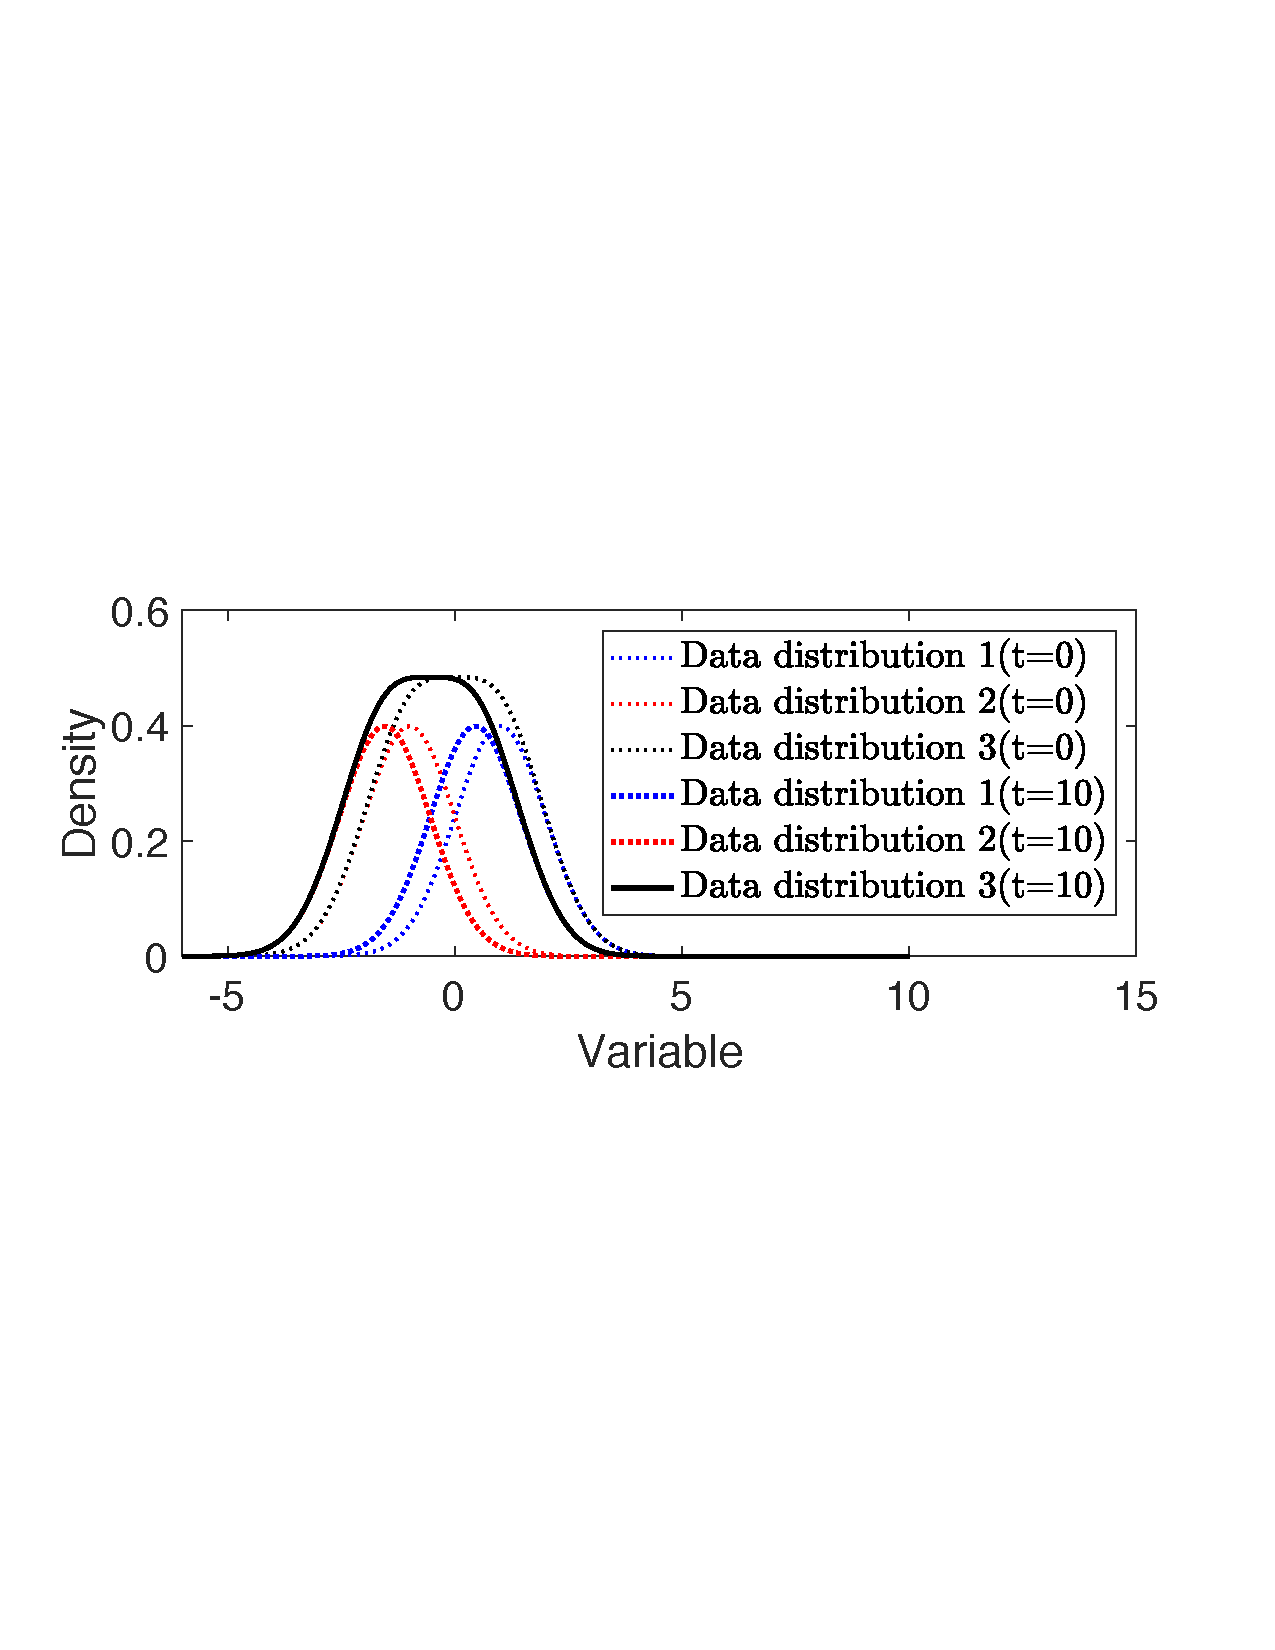
\includegraphics[width=0.7\columnwidth]{figure_dynamics}\label{figure_dynamics}}
\caption{The illustration of the dynmaics caused by the time-varying distributions of data. Data distribution $1$ and $2$ are  Normal distrbutions with $1$ variance and $1+\sin(t)$ mean, and $1$ variance and $-1+\sin(t)$ mean, respectively. Data distribution $3$ is the sum of them, which changes over time. }
\label{figure_illus_dynamics}
\end{figure}


\begin{figure*}[!h]
\setlength{\abovecaptionskip}{0pt}
\setlength{\belowcaptionskip}{0pt}
\centering 
\subfigure[\textit{synthetic data}, $100$ nodes]{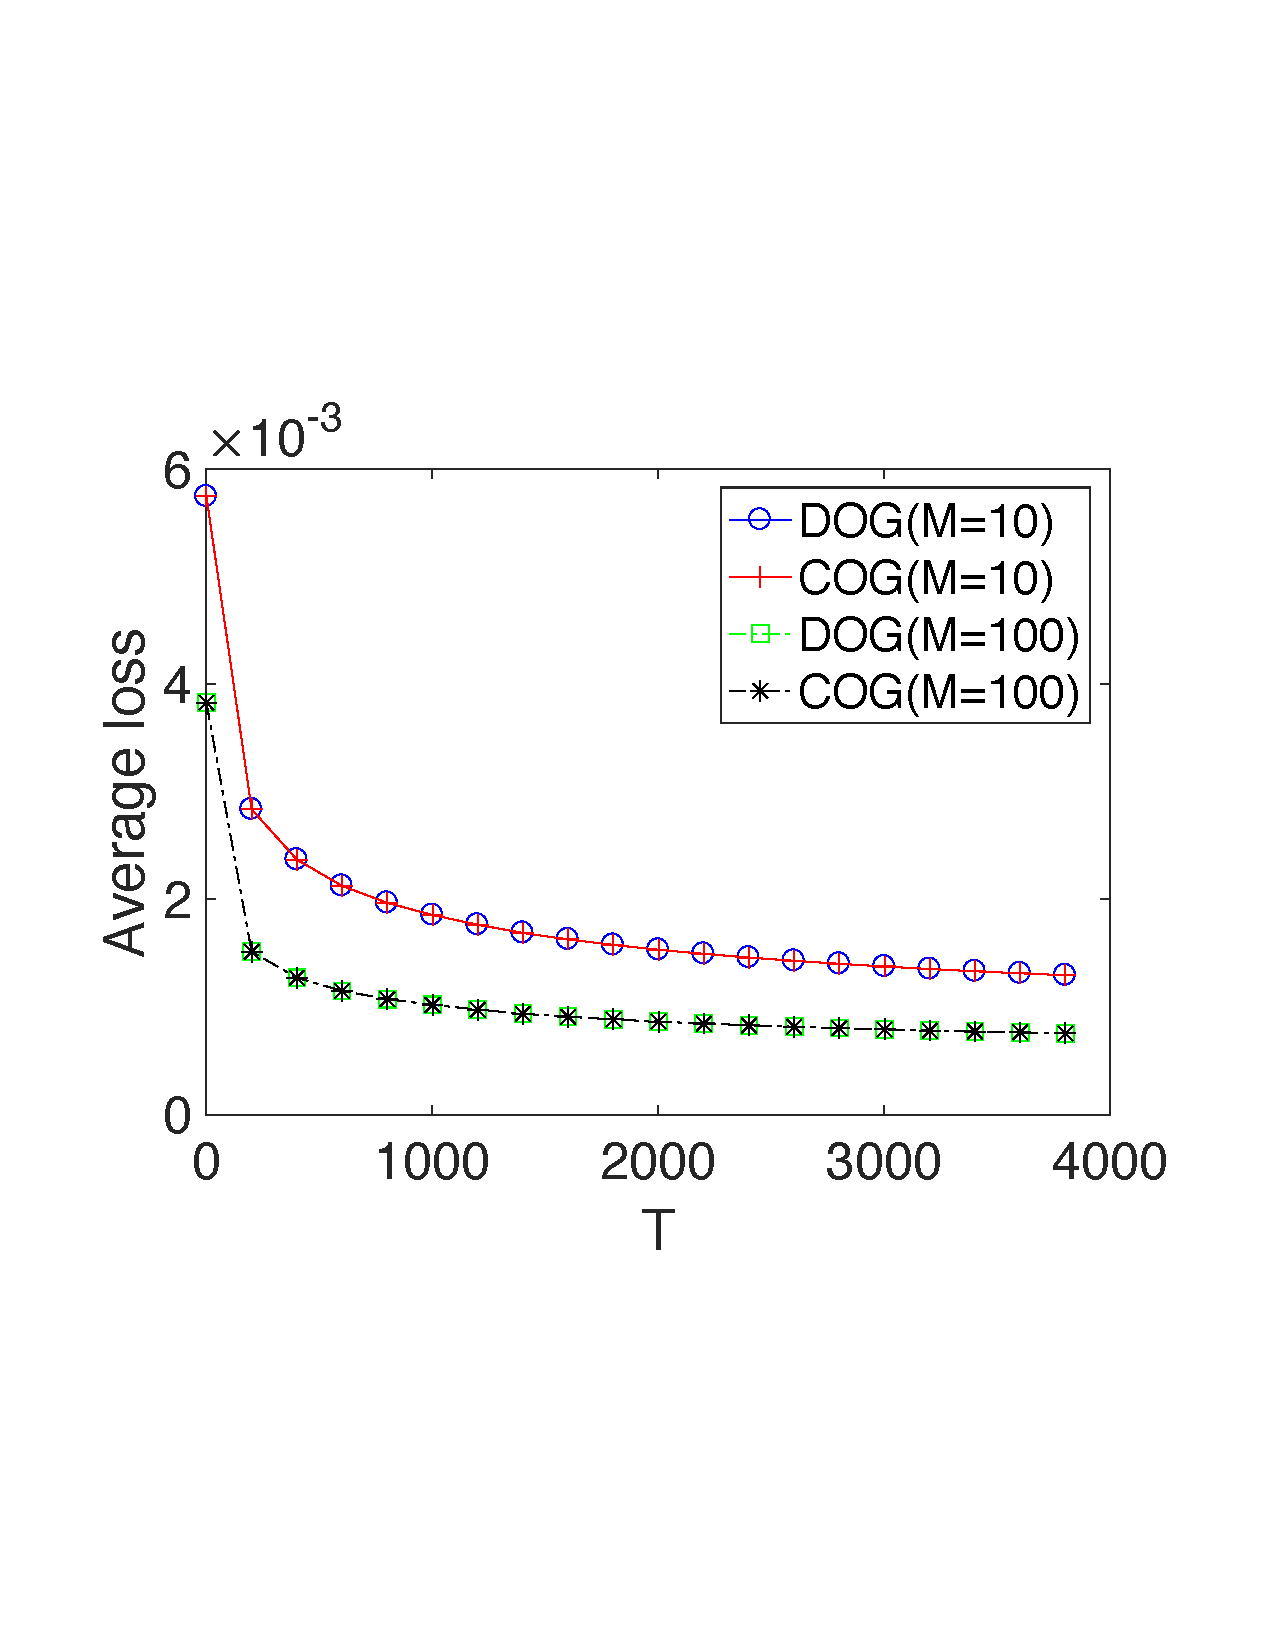
\includegraphics[width=0.48\columnwidth]{figure_decen_cen_ave_loss_iterations}\label{figure_decen_cen_ave_loss_iterations}}
\subfigure[\textit{room-occupancy}, $5$ nodes]{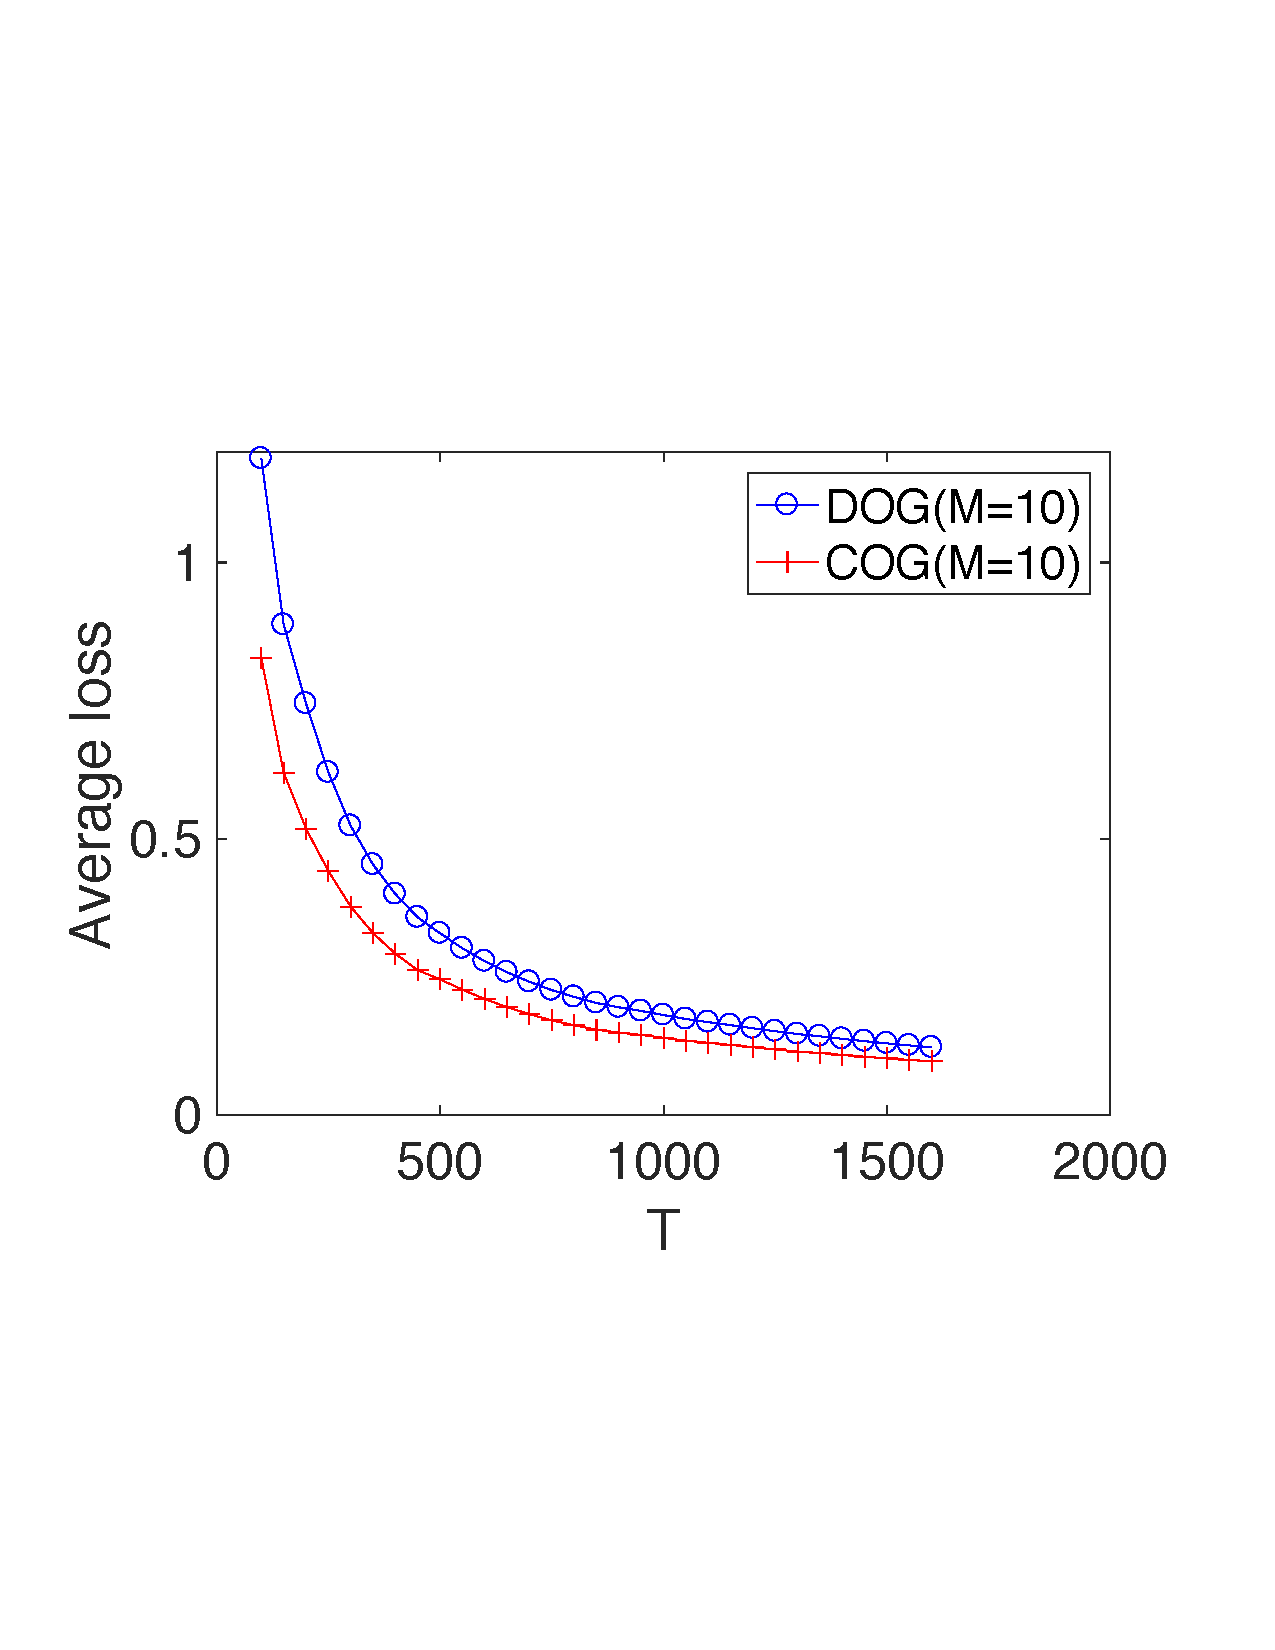
\includegraphics[width=0.48\columnwidth]{figure_decen_cen_ave_loss_iterations_occupancy}\label{figure_decen_cen_ave_loss_iterations_occupancy}}
\subfigure[\textit{usenet2}, $5$ nodes]{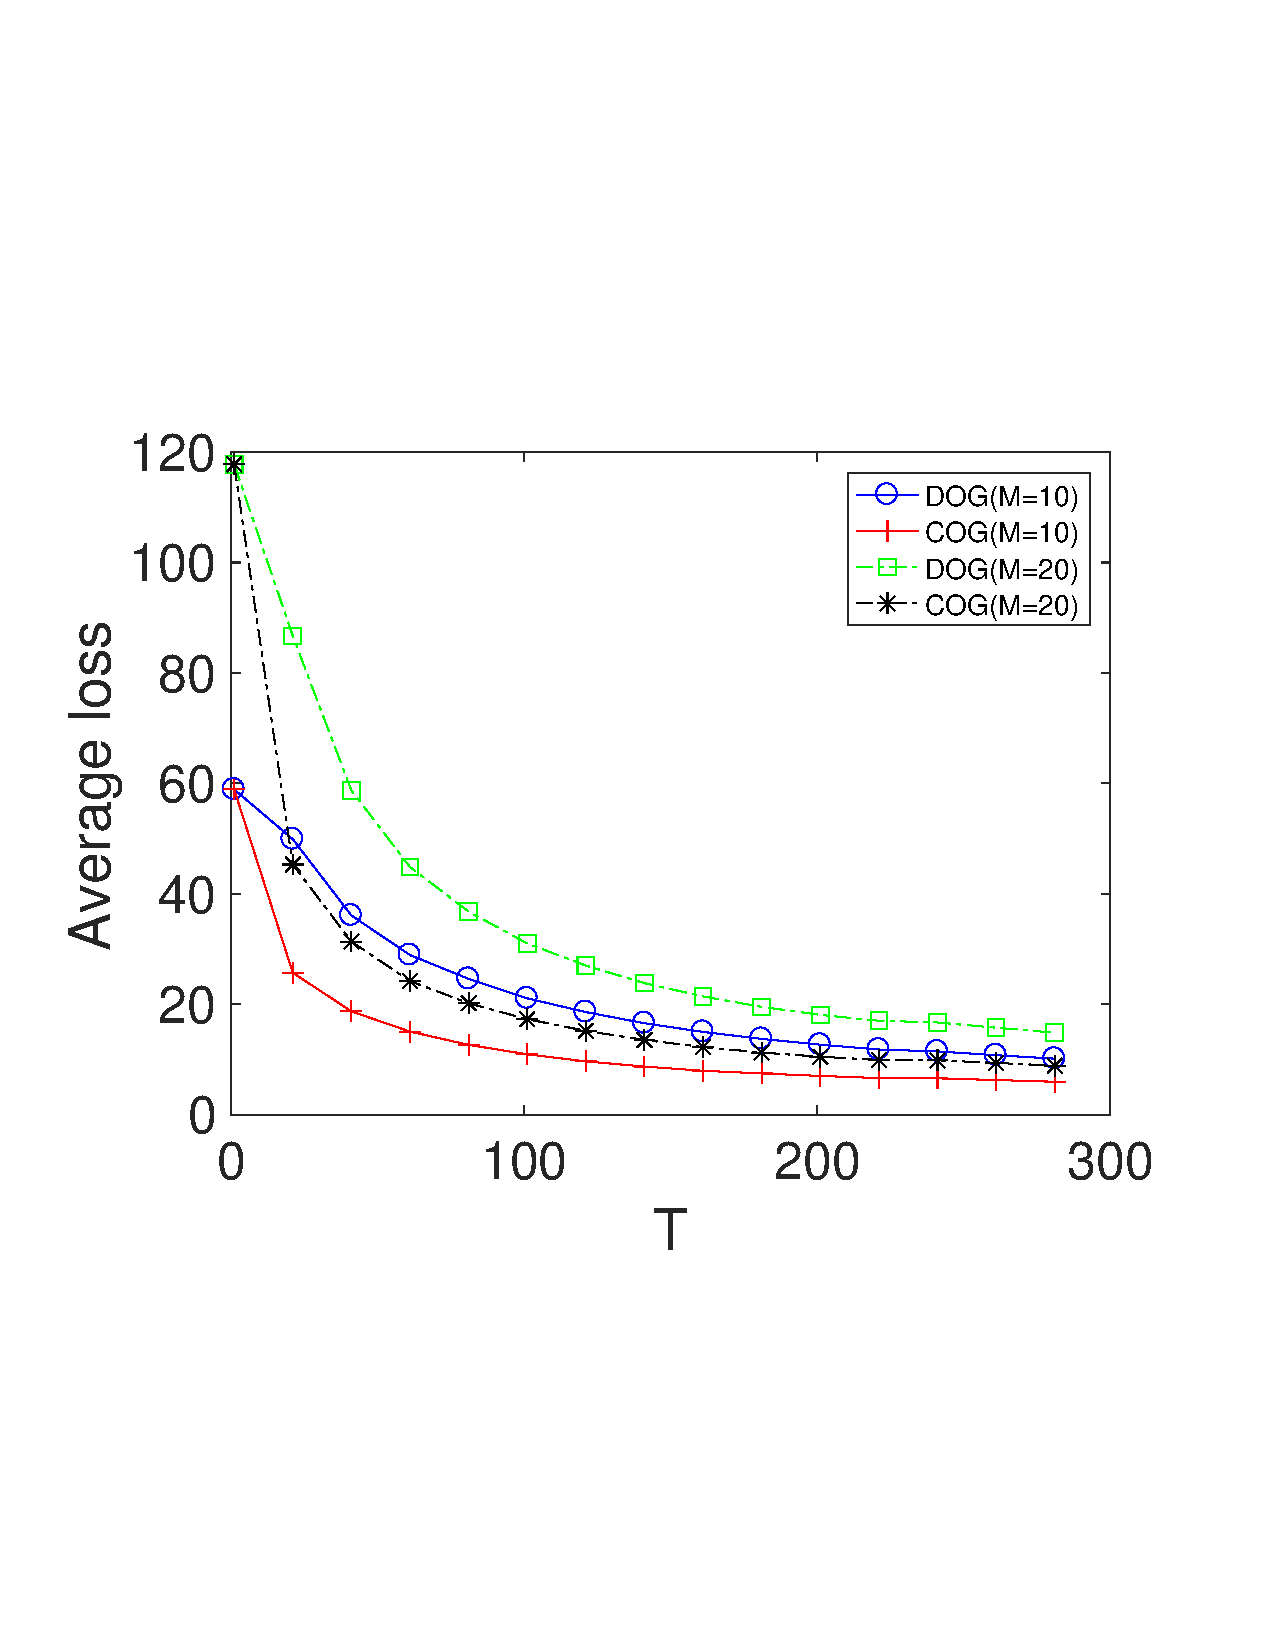
\includegraphics[width=0.48\columnwidth]{figure_decen_cen_ave_loss_iterations_usenet2}\label{figure_decen_cen_ave_loss_iterations_usenet2}}
\subfigure[\textit{spam}, $5$ nodes]{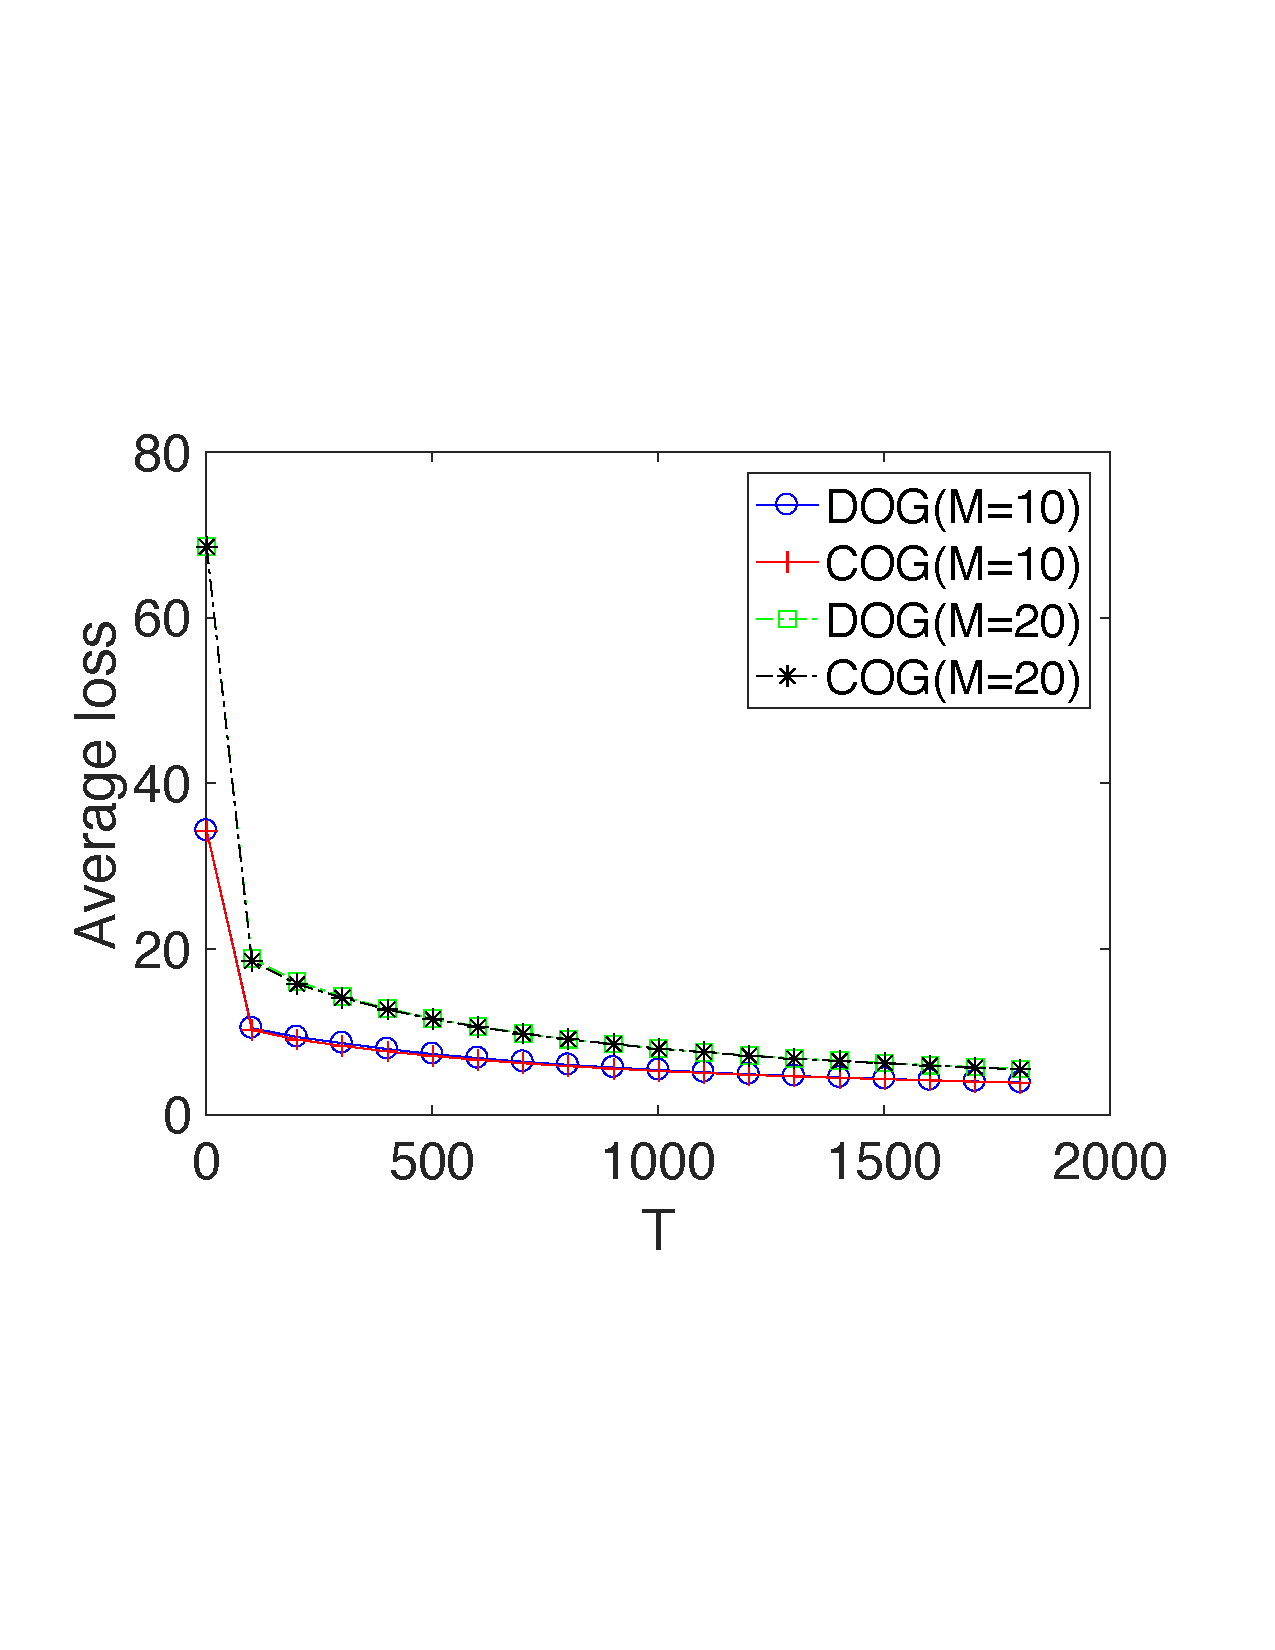
\includegraphics[width=0.48\columnwidth]{figure_decen_cen_ave_loss_iterations_spam}\label{figure_decen_cen_ave_loss_iterations_spam}}
%\subfigure[\textit{usenet2}]{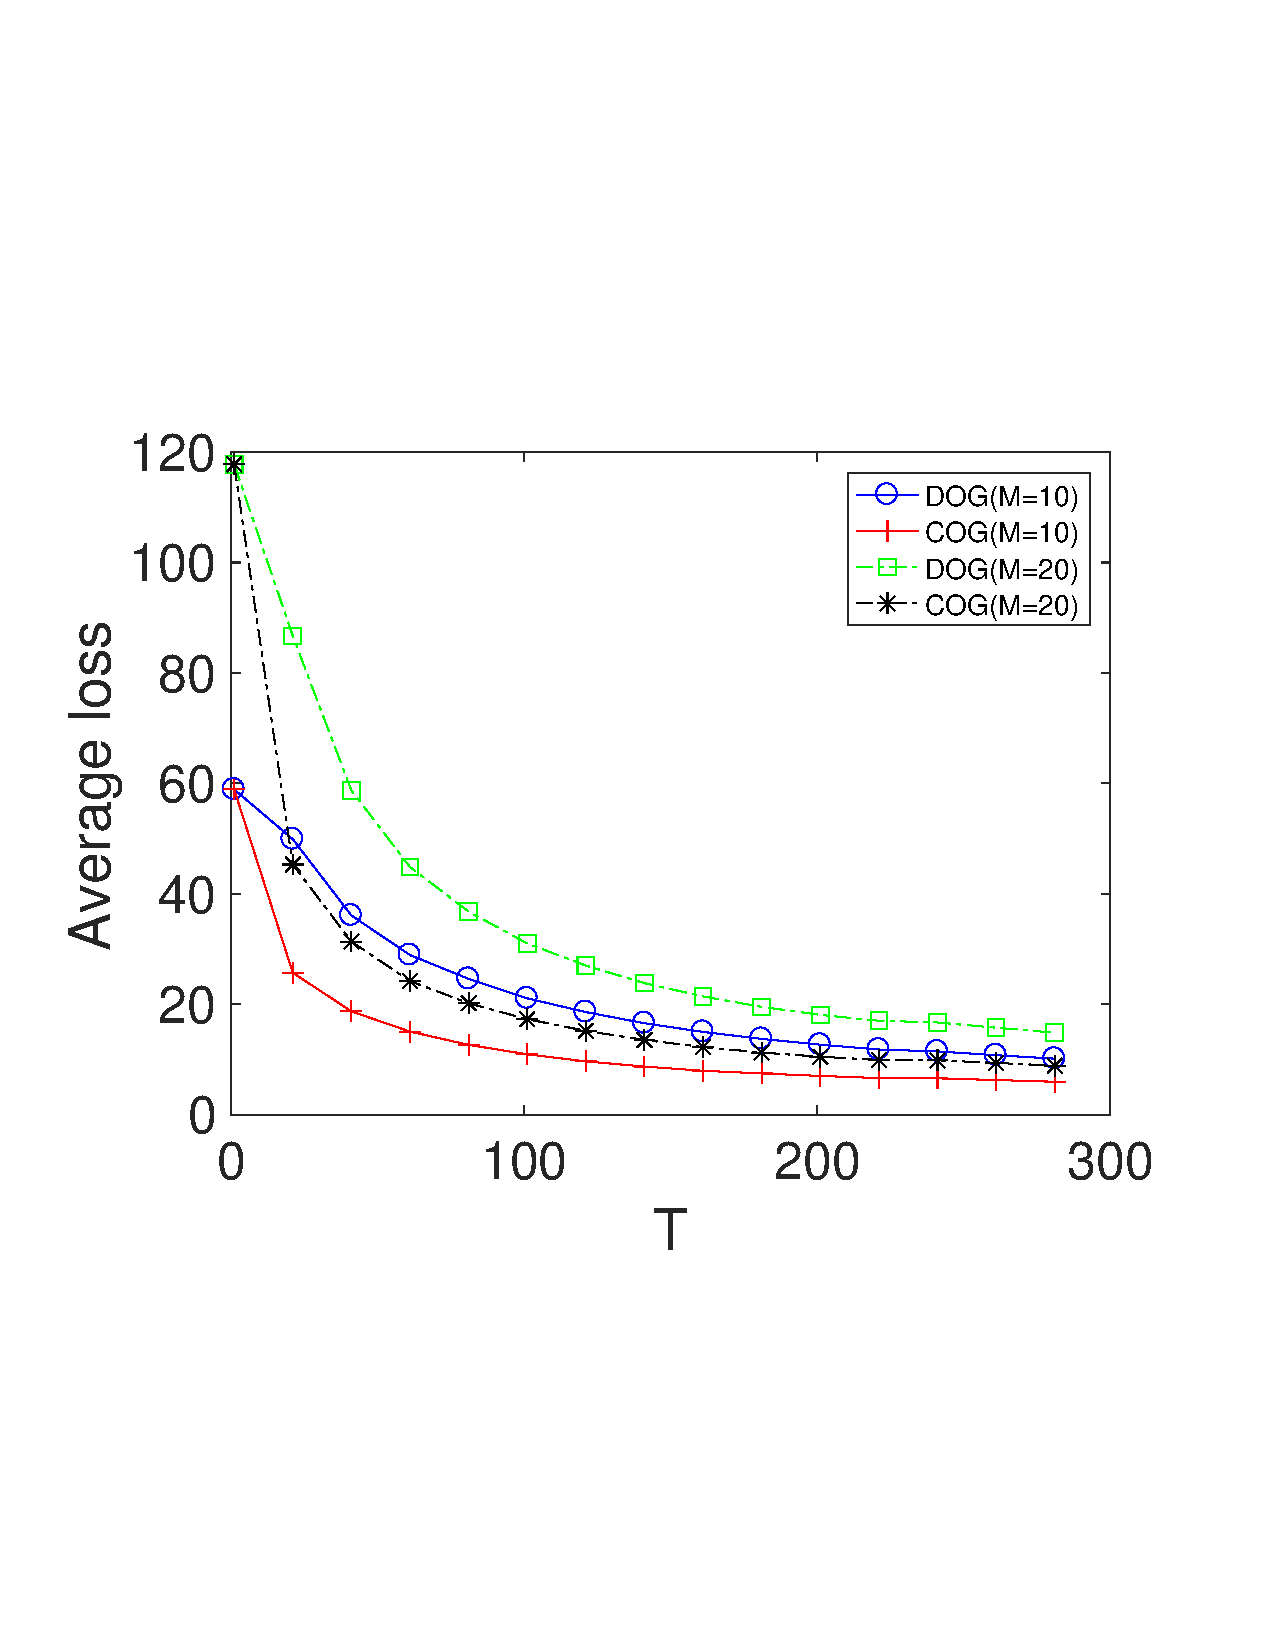
\includegraphics[width=0.32\columnwidth]{figure_decen_cen_ave_loss_iterations_usenet2}\label{figure_decen_cen_ave_loss_iterations_usenet2}}
\caption{The average loss yielded by DOG is comparable to that yielded by COG.}
\label{figure_compare_loss}
\end{figure*}







\textbf{Synthetic data} We generate a data matrix $\A=\A_1 + \A_2+ \cdots + \A_n$, where $\A_i$ is placed on the $i$-th node, and $\A_i=0.1\tilde{\A}_i+0.9\hat{\A}_i$, where $\tilde{\A}_i$ represents the adversary part of data, and $\hat{\A}_i$ represents the stochastic part of data. $\y_{i}\in\{1,-1\}$ is the label of an instance $\hat{\A}_{i,t}$. The dimension of every instance is $d = 10$. Specifically,  elements of $\tilde{\A}_i$ is sampled from the interval $[-0.5+\sin(i),0.5+\sin(i)]$ randomly. Note that $\tilde{\A}_i$ and $\tilde{\A}_j$ with $i\neq j$ are drawn from different distributions. Besides, $\y_{i,t}\in\{1,-1\}$ is generated randomly. When $\y_{i,t}=1$, $\hat{\A}_{i,t}$ is generated by sampling from a time-varying Normal distribution $\hat{\A}_{i,t} \sim N((1+0.5\sin(t))\cdot\1, \I)$. When $\y_{i,t} = -1$, $\hat{\A}_{i,t}$ is generated by sampling from another time-varying Normal distribution $\hat{\A}_{i,t} \sim N((-1+0.5\sin(t))\cdot\1, \I)$. As illustrated in Figure \ref{figure_illus_dynamics}, we use those time-varying distributions of data to simulate the dynamics in the environment, which leads to the change of the optimal learning model over time.  In the setting, dynamic regret is practical and necessary to measure goodness of a learning model. 

\textbf{Real data} We use three real datasets: \textit{room-occupancy}\footnote{\url{https://archive.ics.uci.edu/ml/datasets/Occupancy+Detection+}},  \textit{usenet2}\footnote{\url{http://mlkd.csd.auth.gr/concept_drift.html}}, and a \textit{spam}\footnote{\url{http://mlkd.csd.auth.gr/concept_drift.html}}. \textit{room-occupancy} ia time-series dataset, where the dynamics exists naturally in those practical scenarios. Bothe \textit{usenet2} and \textit{spam} contain ``concept drift" \citep{Katakis:2010:TR}, which is the source of the dynamics.  Thus, the dynamic regret is practial and necessary to measure an online learning method to handle those datasets. 

%Besides, we fetch values of the first feature of every dataset, and then permutate them by the decreasing order. After that, we re-fill the new values to the data matrix to simulate the adversary values. Finally, all values of a feature have been normalized to be zero mean and one variance.
%\begin{itemize}
%\item {\textit{room-occupancy}.} It collects features of a room including temperature, humidity, light, and CO2 for every minute between 02/02/2015 and 02/10/2015. Label of an instance is whether the room is occupied. Our goal is to learn a classification model to make a decision whether the room is occupied by using those features.   
%\item {\textit{usenet2}.} It is an online retail dataset, which contains all transactions occurring between 01/12/2010 and 09/12/2011 for a UK-based and registered non-store online retail. We use three features, that is, \textit{whether a transaction is cancelled}, \textit{quantity}, and \textit{unit price}. We need to train a binary clssification model to make a decision whether a customer is coming from United Kingdom. 
%\item {\textit{BeijingPM2.5}.} It collects some weather features, e.g., teperature and pressure, and the PM2.5 data of US Embassy in Beijing hourly between 01/01/2010 and 12/31/2014. When the PM 2.5 index is larger than $100$, the air quality is \textit{bad}, otherwise, \textit{good}. We want to train a binary clssification model to make a decision whether the air quality is good accoring to features such as temperature and pressure.   \textit{BeijingPM2.5}\footnote{\url{https://archive.ics.uci.edu/ml/datasets/Beijing+PM2.5+Data}},
%\item {\textit{spam}.} Every instance in the dataset is an email, where the frequence of every word in the dictionary is collected. But, the distribution of words changes over time, which is denoted by \textit{concept drift} \citep{Katakis:2010:TR}. We want to learn a classification model to make a decision whether an email is a spam. 
%\end{itemize}


\subsection{Results}

First, we want to test whether DOG has a comparable performance with COG. We simulate a decentralized network consisting of $100$ nodes to handle the synthetic data, and a network consisting of $5$ nodes to handle the real data. Those nodes are connected by using a ring topology.  As shown in Figure \ref{figure_compare_loss}, both DOG and COG are effective to optimize the decision variable, and they have very similar performance. 



Second, we want to varify whether DOG has a good performance with the increase of the network size. As shown in Figure \ref{figure_compare_network_size}, the performance of DOG is not sensitive to the network size, which confirms our theoretical result, that is, the average regret $\frac{1}{nT}\EE_{\Xi_{n,T}\sim \Dcal_{n,T}}\sum_{i=1}^n\sum_{t=1}^T \lrincir{ f_{i,t}(\x_{i,t};\xi_{i,t}) - f_{i,t}(\x_t^{\ast}) }$ does not increase over the number of nodes. 




\begin{figure*}[!h]
\setlength{\abovecaptionskip}{0pt}
\setlength{\belowcaptionskip}{0pt}
\centering 
\subfigure[\textit{synthetic data}, ring topology]{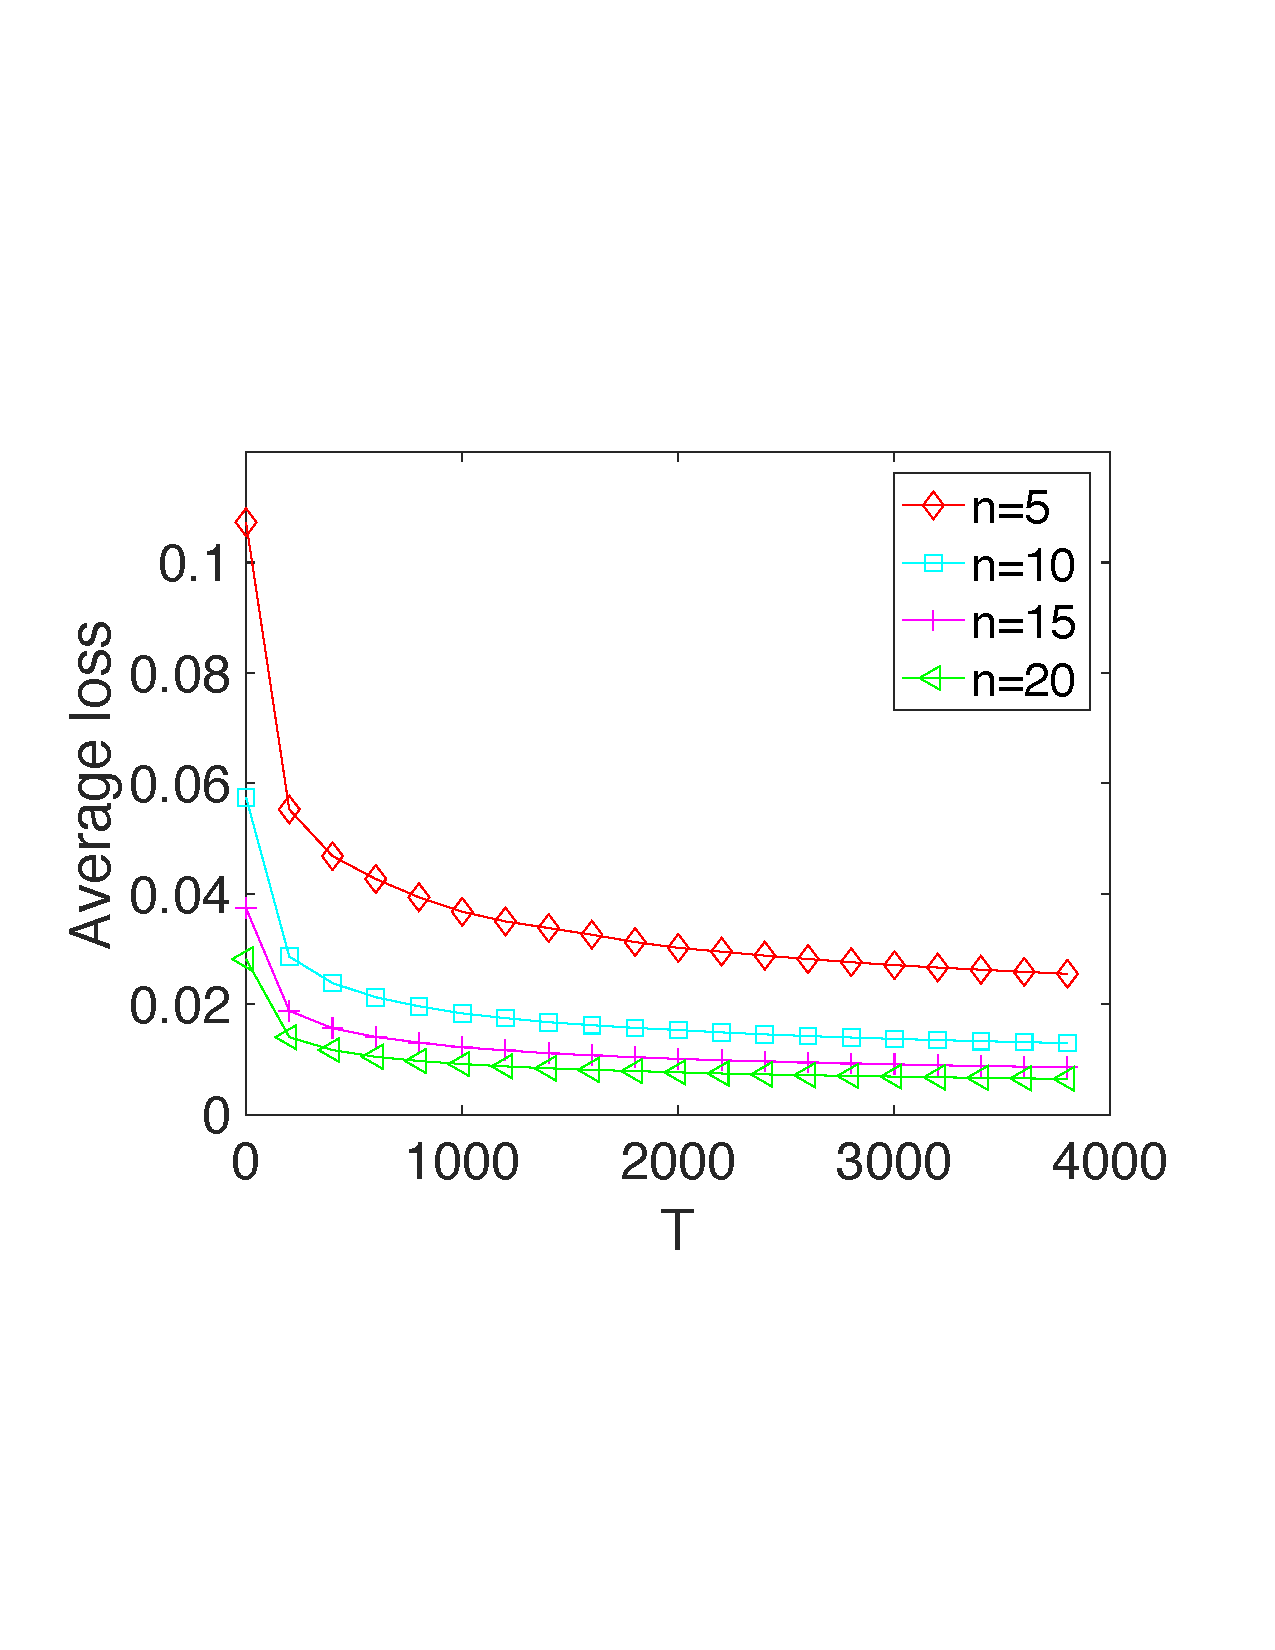
\includegraphics[width=0.48\columnwidth]{figure_decen_cen_ave_loss_nodes}\label{figure_decen_cen_ave_loss_nodes}}
\subfigure[\textit{room-occupancy}, ring topology]{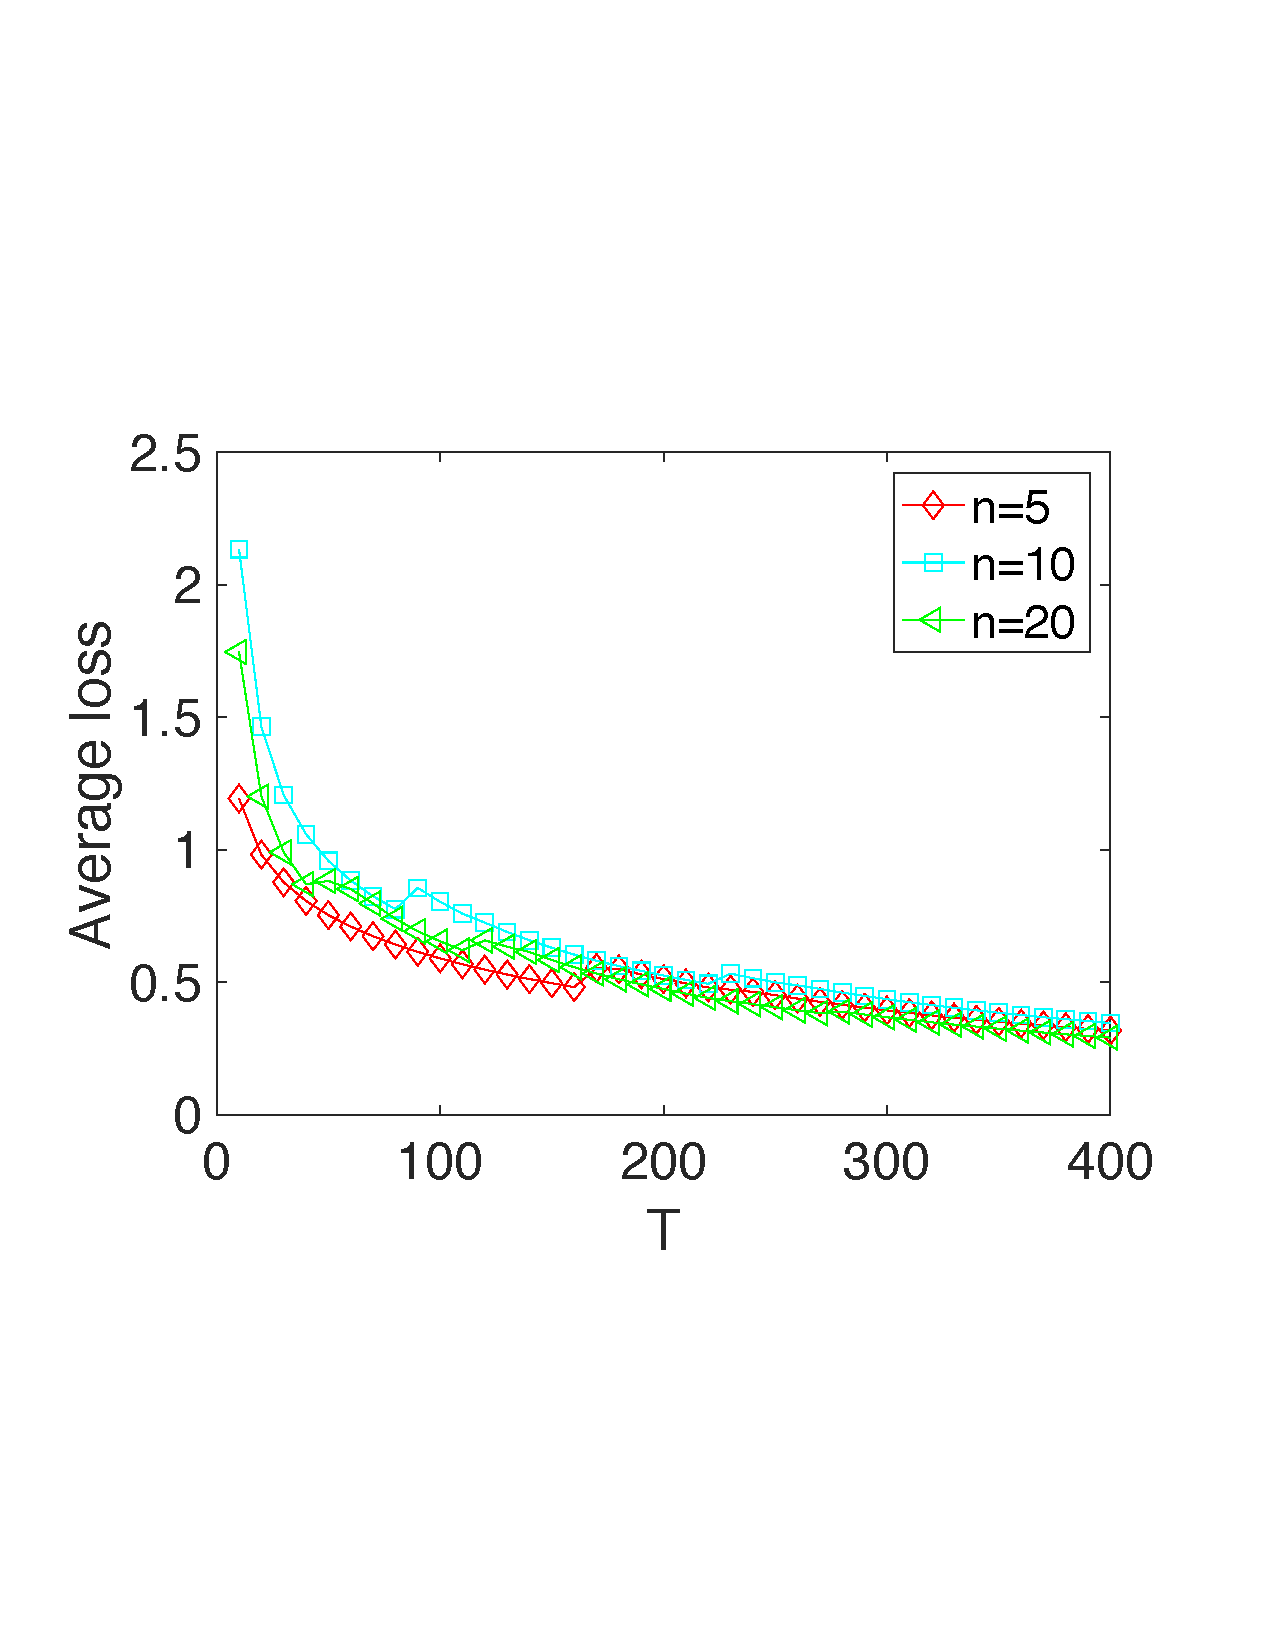
\includegraphics[width=0.48\columnwidth]{figure_decen_cen_ave_loss_nodes_occupancy}\label{figure_decen_cen_ave_loss_nodes_occupancy}}
\subfigure[\textit{usenet2}, ring topology]{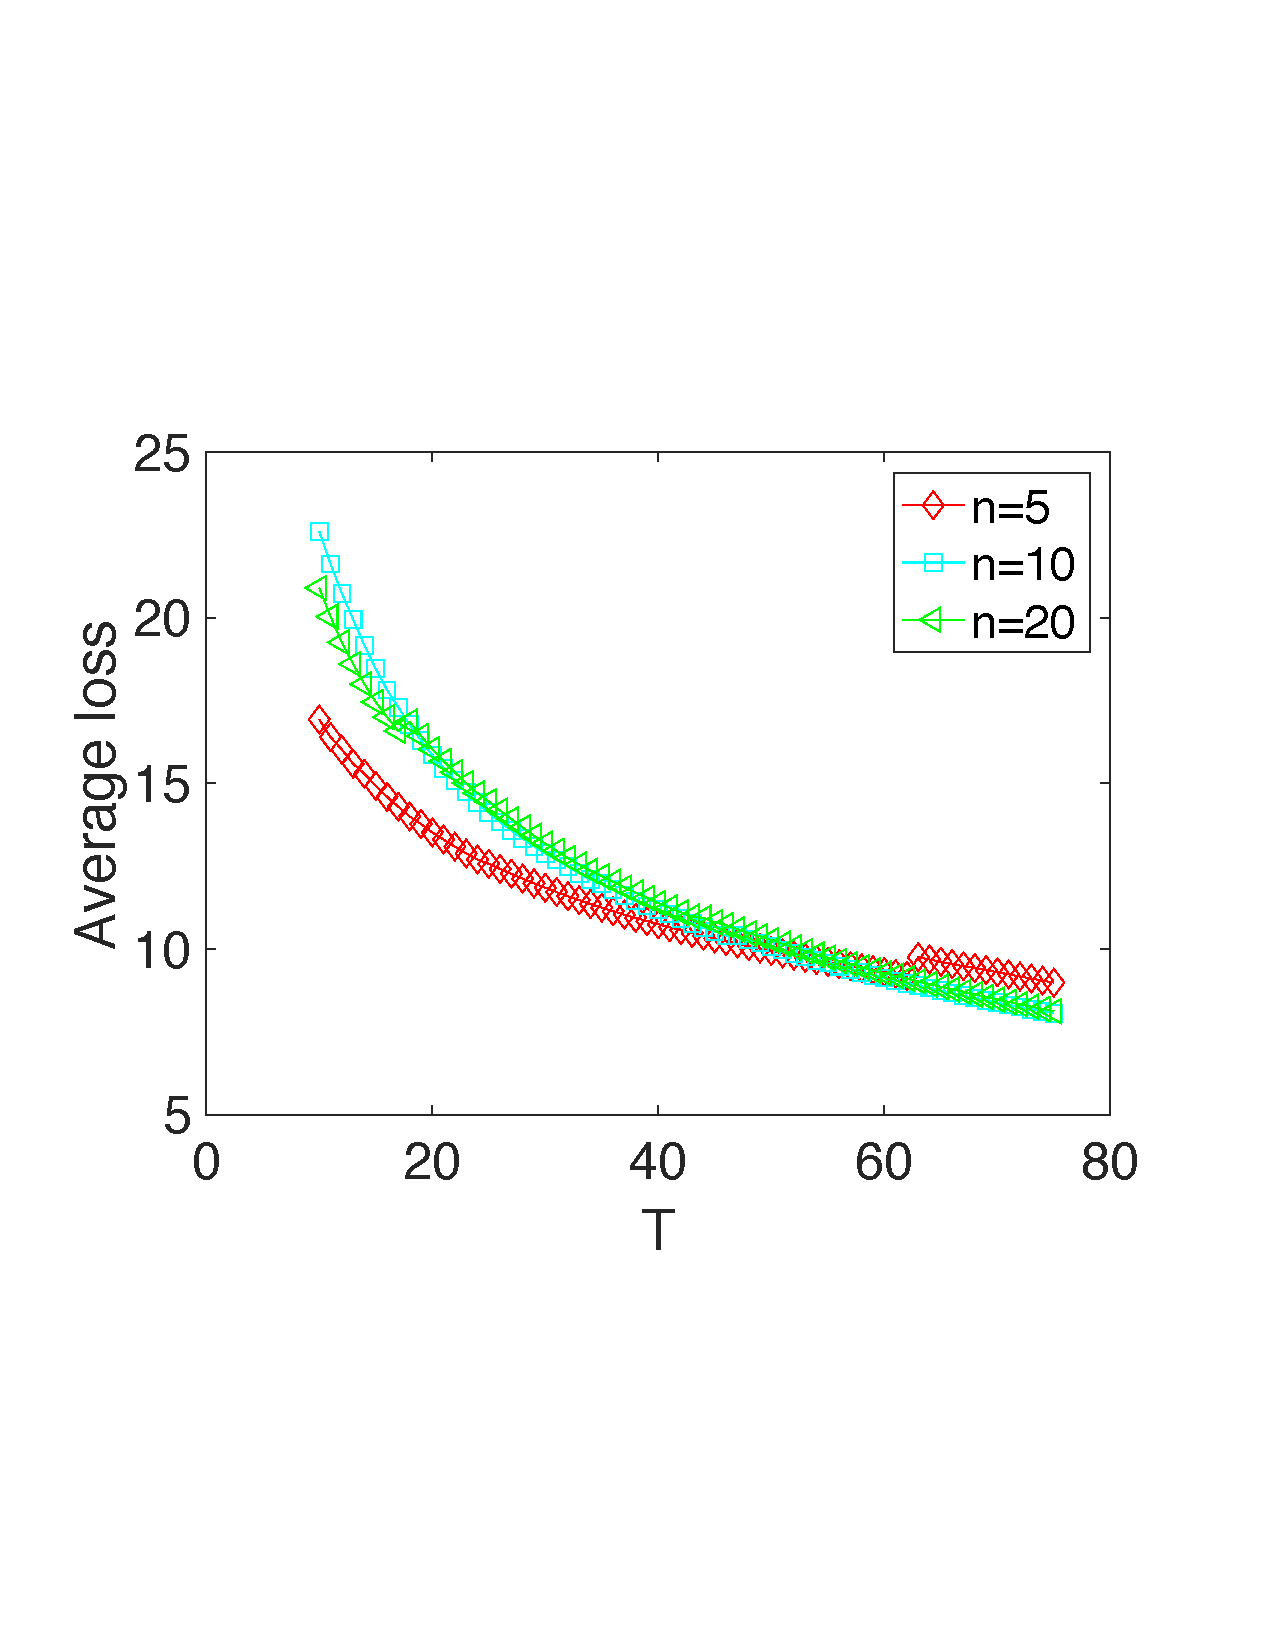
\includegraphics[width=0.48\columnwidth]{figure_decen_cen_ave_loss_nodes_usenet2}\label{figure_decen_cen_ave_loss_nodes_usenet2}}
\subfigure[\textit{spam}, ring topology]{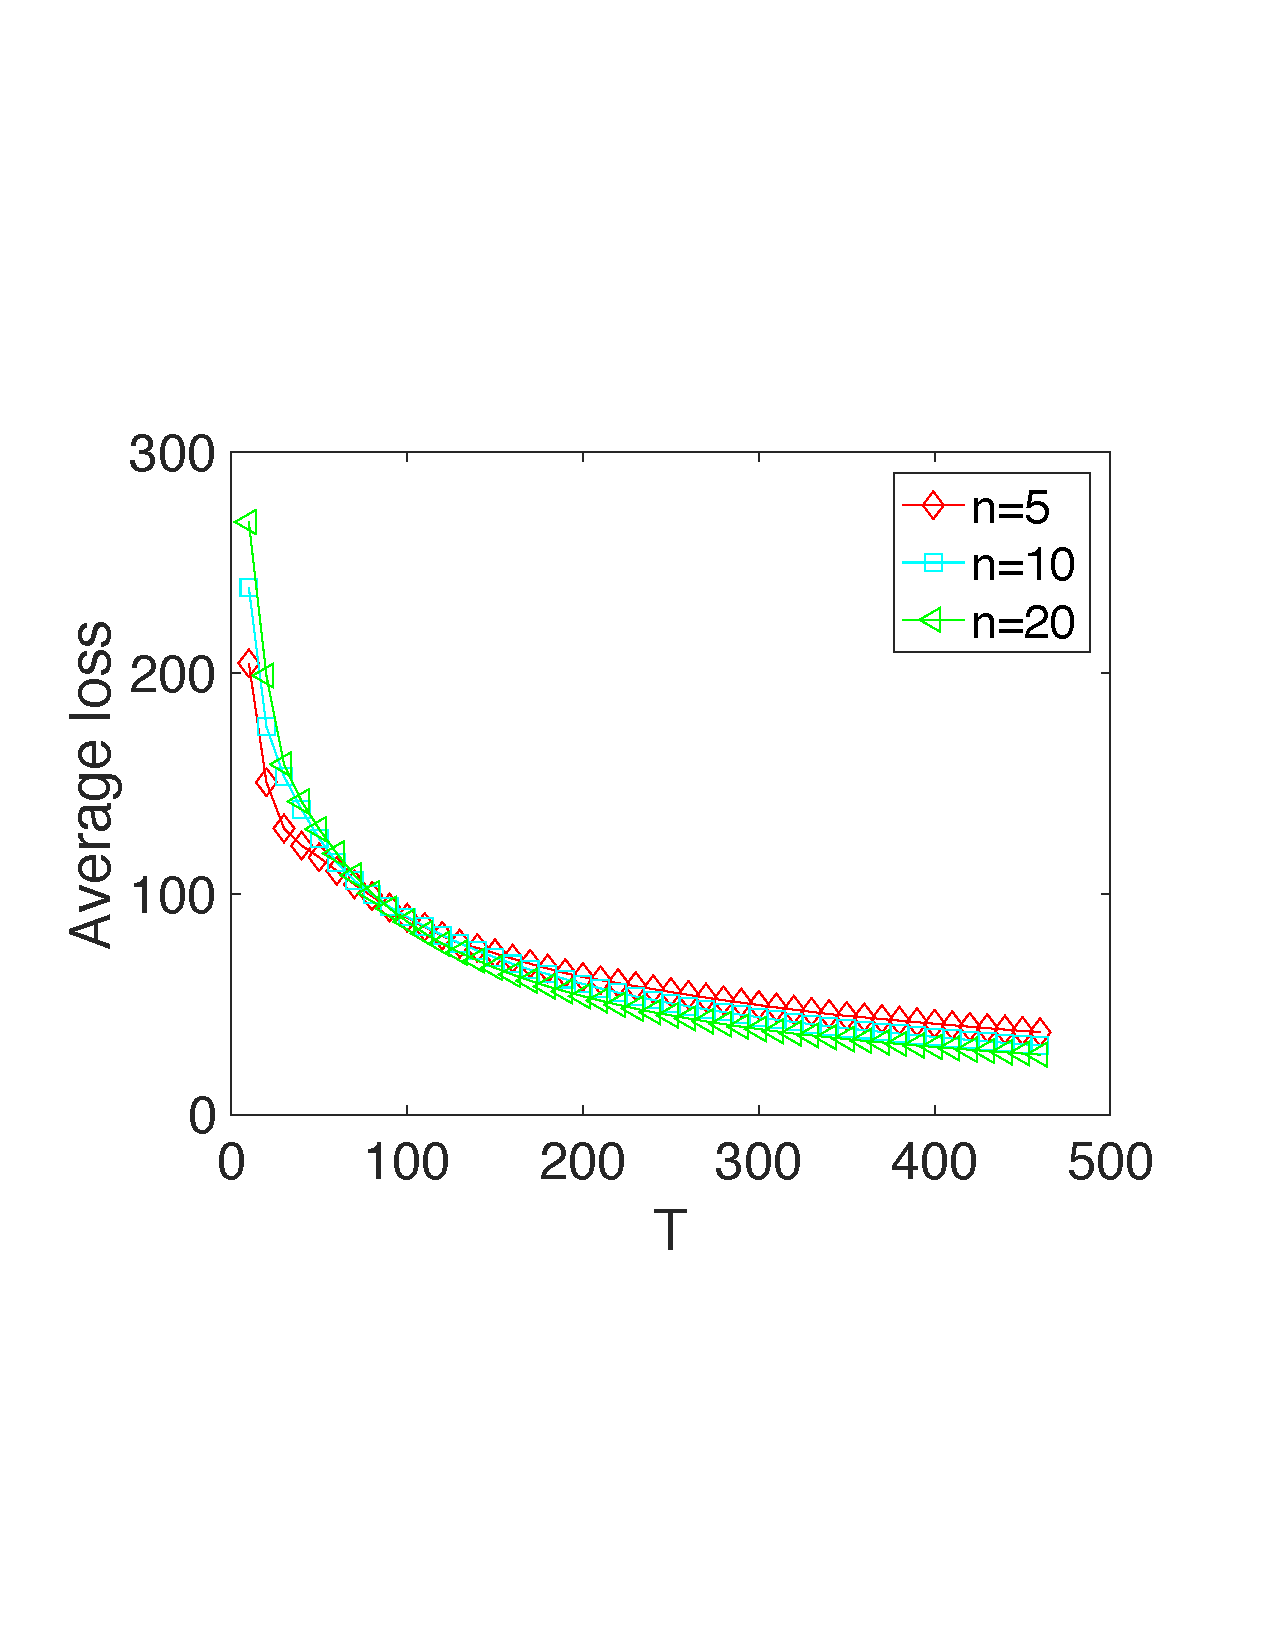
\includegraphics[width=0.48\columnwidth]{figure_decen_cen_ave_loss_nodes_spam}\label{figure_decen_cen_ave_loss_nodes_spam}}
\caption{The average loss yielded by DOG is insensitive to the network size.}
\label{figure_compare_network_size}
\end{figure*}


Third, we want to test whether the performance of DOG is sensitive to the topology of the network. We generate four different topologies. Besides the ring topology, the \textit{Fully connected} means all nodes are connected, where DOG de-generates to be COG. The topology  \textit{WattsStrogatz} represents a Watts-Strogatz small-world graph. There is a parameter can be tuned, e.g., $0.5$ or $1$ in the legend of Figure \ref{figure_compare_topology}, to control the number of random edges.  As illustrated in Figure \ref{figure_compare_topology}, \textit{Fully connected} has the best performance because that $\rho = 0$ in the topology, and $\rho>0$ in other topologies.  



\begin{figure*}[!h]
\setlength{\abovecaptionskip}{0pt}
\setlength{\belowcaptionskip}{0pt}
\centering 
\subfigure[\textit{synthetic data}, $100$ nodes]{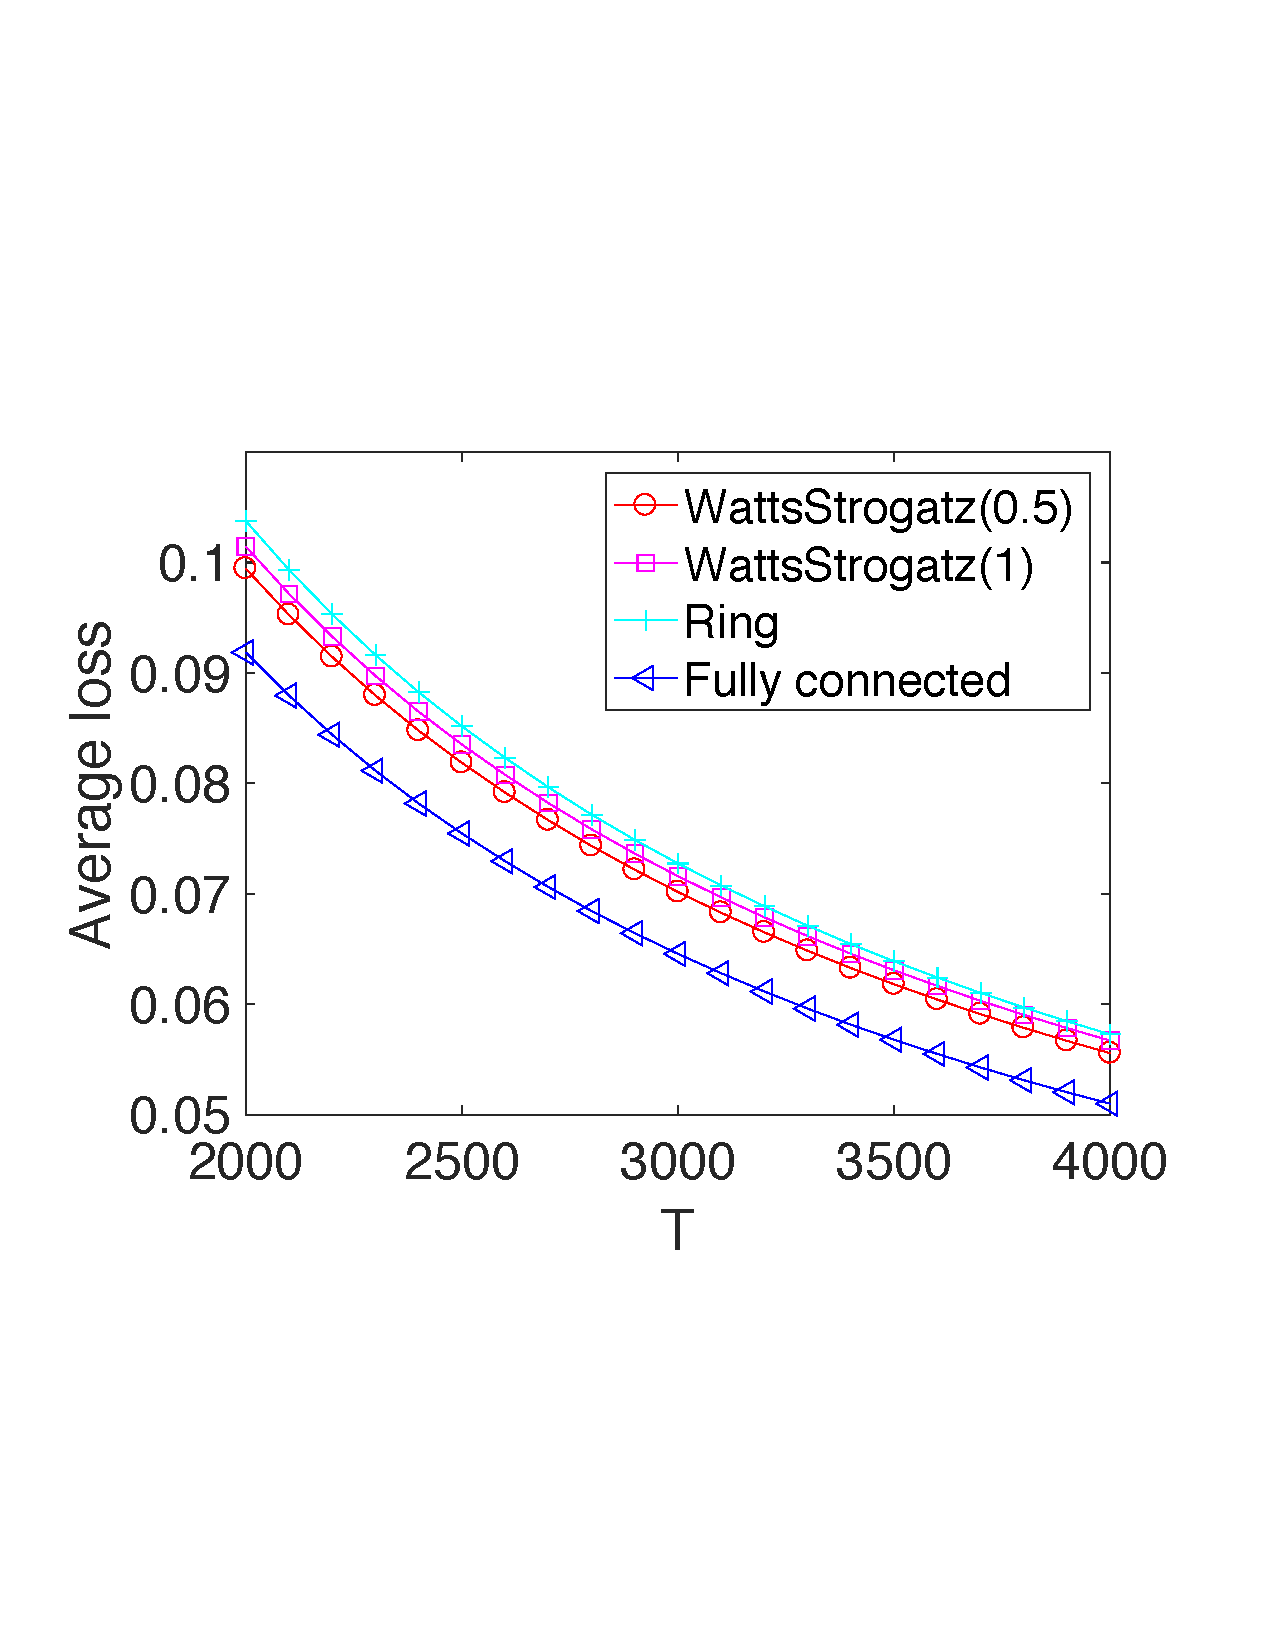
\includegraphics[width=0.48\columnwidth]{figure_decen_cen_ave_loss_iterations_net_types}\label{figure_decen_cen_ave_loss_iterations_net_types}}
\subfigure[\textit{room-occupancy}, $20$ nodes]{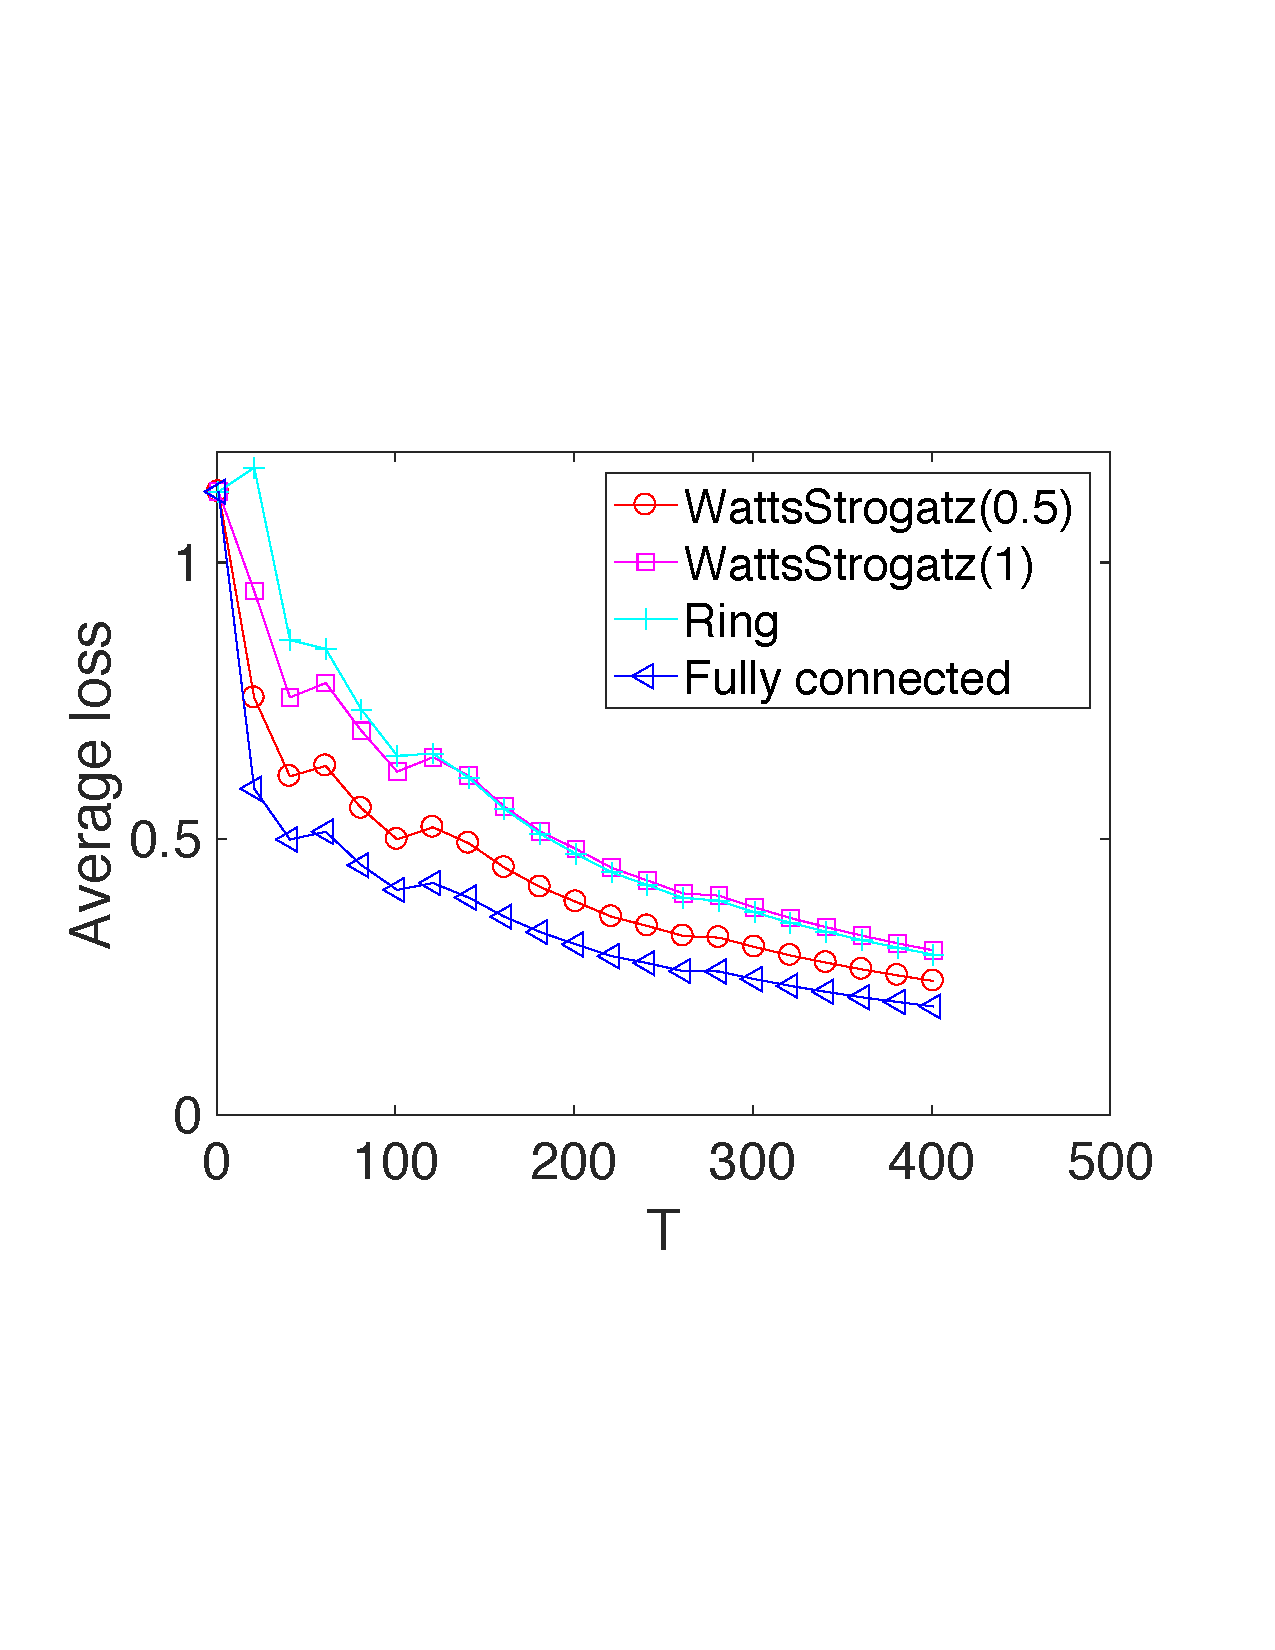
\includegraphics[width=0.48\columnwidth]{figure_decen_cen_ave_loss_iterations_net_types_occupancy}\label{figure_decen_cen_ave_loss_iterations_net_types_occupancy}}
\subfigure[\textit{usenet2}, $20$ nodes]{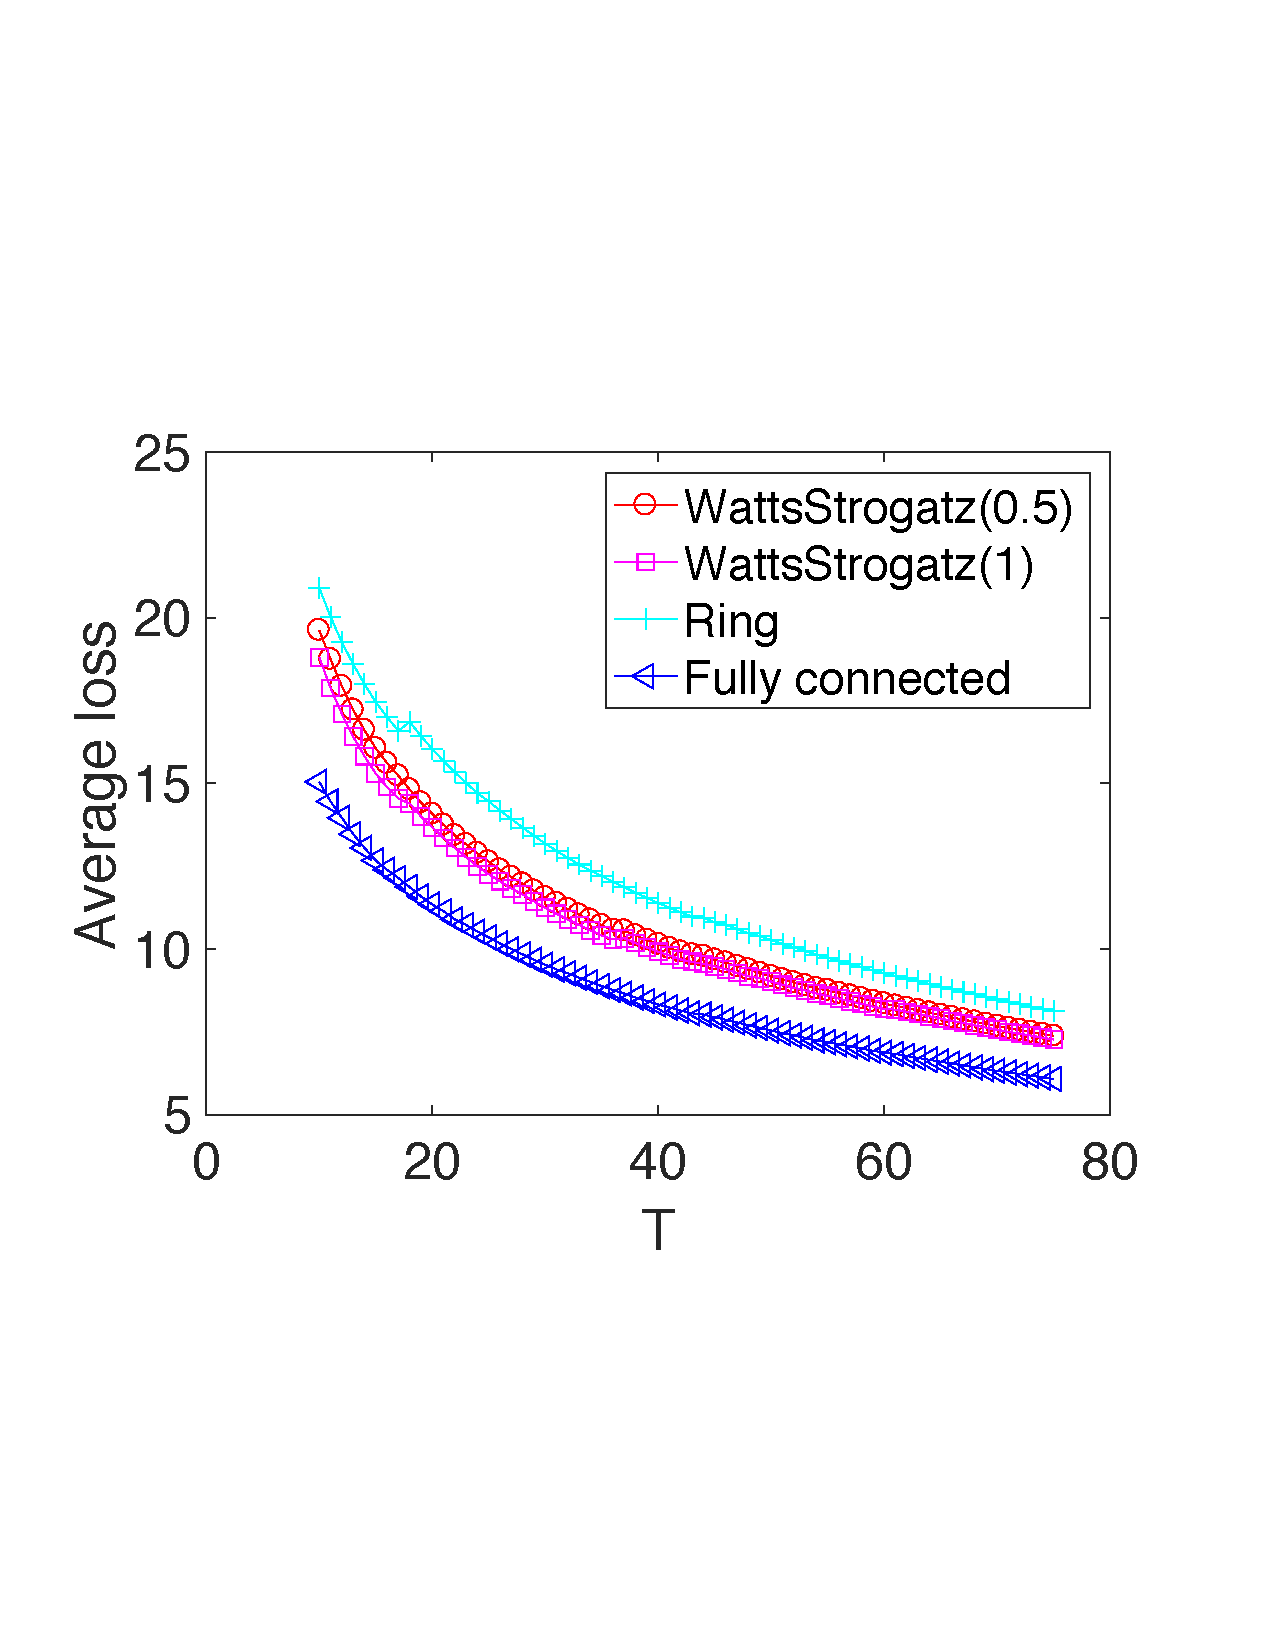
\includegraphics[width=0.48\columnwidth]{figure_decen_cen_ave_loss_iterations_net_types_usenet2}\label{figure_decen_cen_ave_loss_iterations_net_types_occupancy}}
\subfigure[\textit{spam}, $20$ nodes]{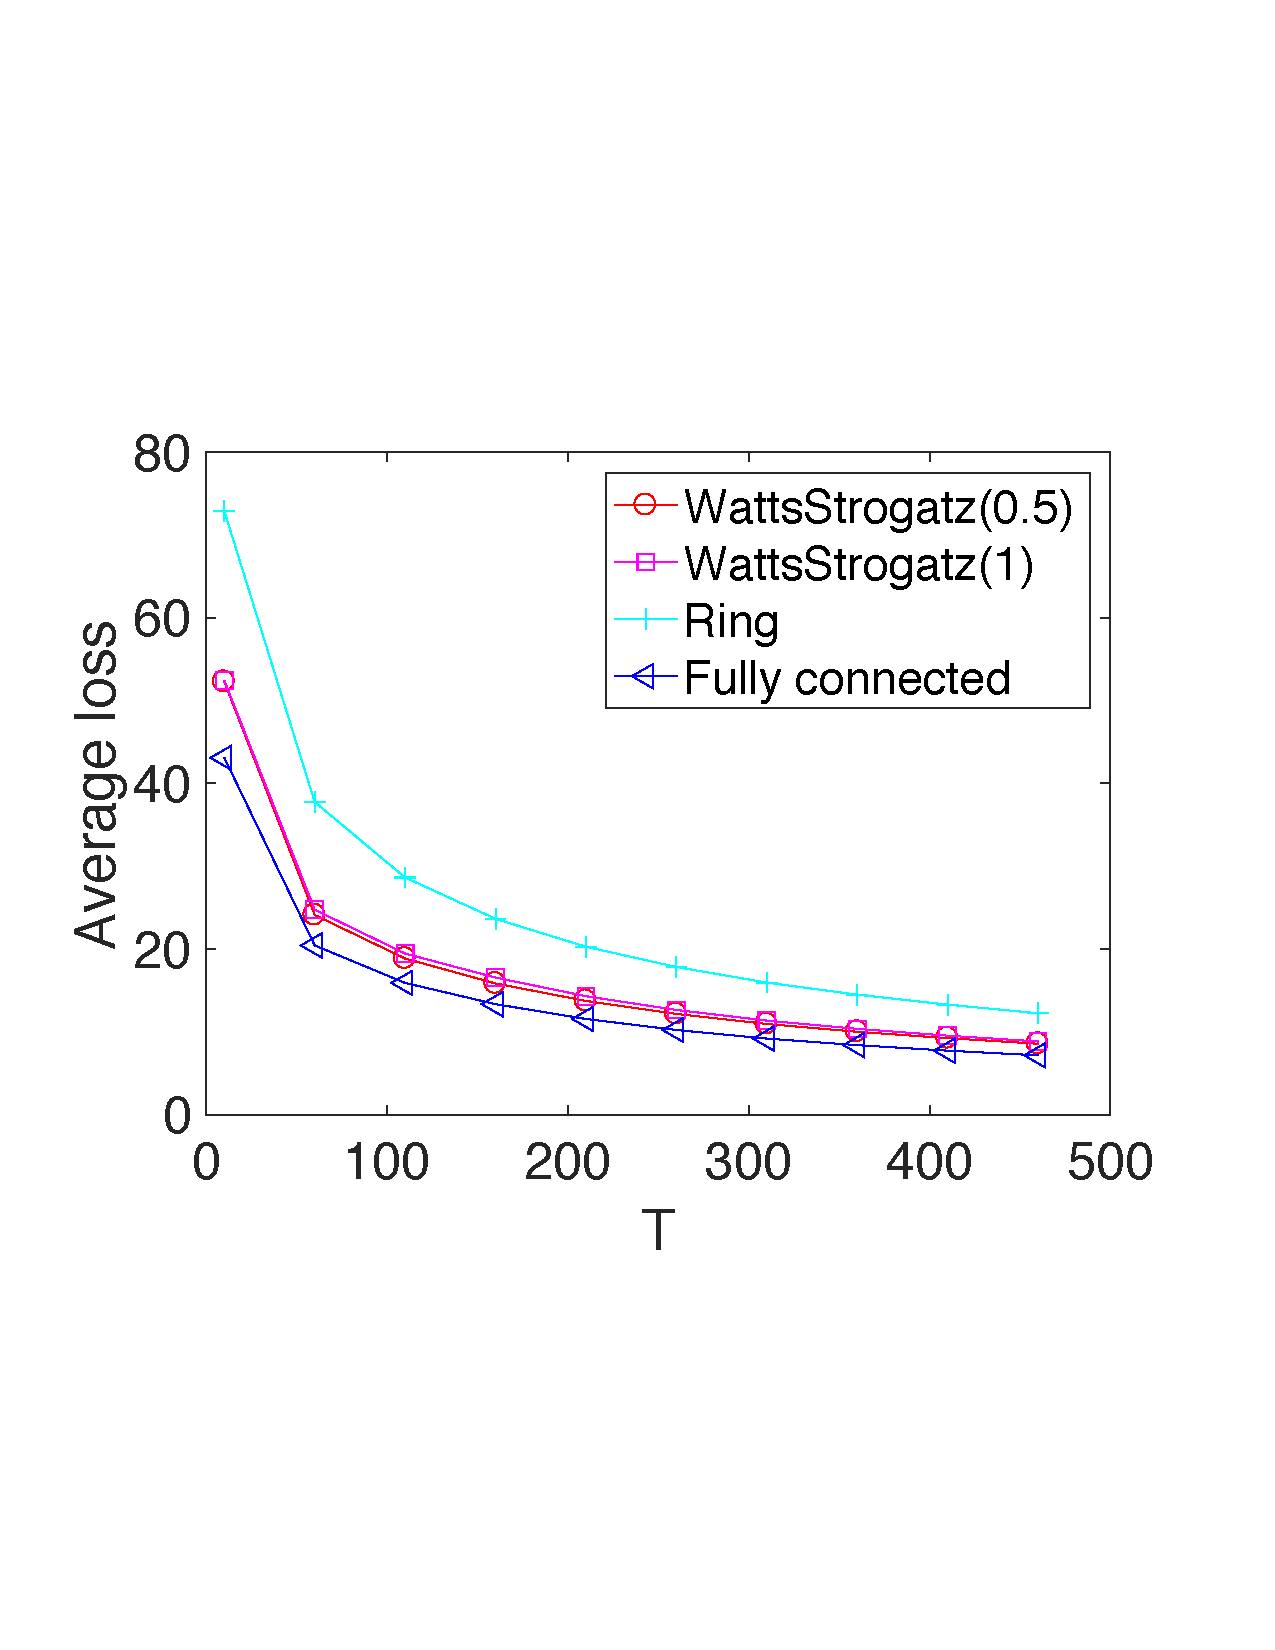
\includegraphics[width=0.48\columnwidth]{figure_decen_cen_ave_loss_iterations_net_types_spam}\label{figure_decen_cen_ave_loss_iterations_net_types_spam}}
\caption{The average loss yielded by DOG is insensitive to the topology of the network.}
\label{figure_compare_topology}
\end{figure*}




\section{Conclusion}
We investigate a new online learning problem in a decentralized network, where the loss incurs by both adversary and stochastic data.  We provide a new analysis framework, which achieves sublinear regret. Extensive empirical studies varify the theoretical result. 


%\section*{References}
\bibliography{reference}

\bibliographystyle{abbrvnat}







\end{document}